Ajustar y optimizar es un proceso iterativo susceptible a la automatización.
Esta fase se refiere a la búsqueda de arquitectura (tamaño de las capas, número
de neuronas) e hiperparámetros (tamaño de lote, tasa de aprendizaje) que harán
que el modelo elegido en la fase anterior alcance su mayor potencial y
posiblemente solucione el problema. Cabe mencionar que todos estos pasos no
garantizan converger a una solución específica, y puede que se tenga que pasar
por varias iteraciones de la metodología para encontrar alguna satisfactoria.

Los hiperparámetros pueden ser exclusivos para cada algoritmo, sin embargo, las
técnicas de búsqueda de hiperparámetros son universales (Búsqueda reticular,
búsqueda aleatoria, bayesiana, metaheurísticas\footnote{Algoritmos de
optimización especializados en espacios no convexos.}). Si los recursos
computacionales lo permiten, utilizar ensamblaje de modelos es mejor que un solo
modelo.

Al ser la fase más computacionalmente intensiva de toda la metodología, esta
fase tiende a ser tardada, normalmente de muchas horas. Al finalizar tendremos
no solo el mejor modelo, sino una evaluación del mismo que nos permitirá avanzar
a la culminación del proceso, o comenzar el proceso una vez más si el
rendimiento no es satisfactorio.

Se procederá realizar tres experimentos. Cada uno de ellos será entrenado por el
mismo algoritmo de entrenamiento y tendrá sus hiperparámetros particulares y se
someterán a varias pruebas y validaciones:

\begin{enumerate}
    \item{\textbf{Clasificación binaria:}} Clasificar las imágenes citológicas
    en normales y anormales.
    \item{\textbf{Clasificación multi-clase:}} Clasificar las imágenes en las
    siete clases del sistema \emph{Bethesda}. Esta será el modelo que llegará a
    la solución final y por ello es el que lleva mayor cantidad de análisis.
    \item{\textbf{Segmentación semántica:}} Segmentar cada pixel de la imagen
    citológica en dos clases: núcleo o el resto (citoplasma o fondo).
\end{enumerate}

\subsection{Implementar validación cruzada}

Se cuenta con un archivo \emph{.csv} que concentra la ruta de la imagen, la clase y la
categoría a la que pertenece. Implementar validación cruzada se reduce a dividir
aleatoriamente los índices de cada fila de tal archivo. Para ello se utilizará
el módulo \emph{Pandas} para manejar los datos tabulares para implementar la
validación cruzada mediante el módulo \emph{Sklearn} y su función
\mintinline{latex}{Kfold}.

La fase de segmentación semántica no cuenta con gráfica de validación cruzada ya
que no se dividen las imágenes por clases.

Se decidió una \mintinline{latex}{K = 10} ya que tienen el mejor compromiso
entre sesgo y varianza. Este proceso es muy tardado pero para asegurar una
estimación precisa del error de generalización, se decidió que era la mejor
opción para validar este trabajo.

\subsubsection{Clasificación binaria}

En la~\autoref{fig:kfold} se representa la planeación de la validación cruzada,
las dos clases, sus índices y como el algoritmo escoge aleatoriamente
subconjuntos (índices) en cada iteración para asegurar una correcta validación
del algoritmo. Se decidió por 10 iteraciones debido a la complejidad
computacional, tardando esta fase 22 horas en completarse.

\begin{figure}[H]
    \centering
    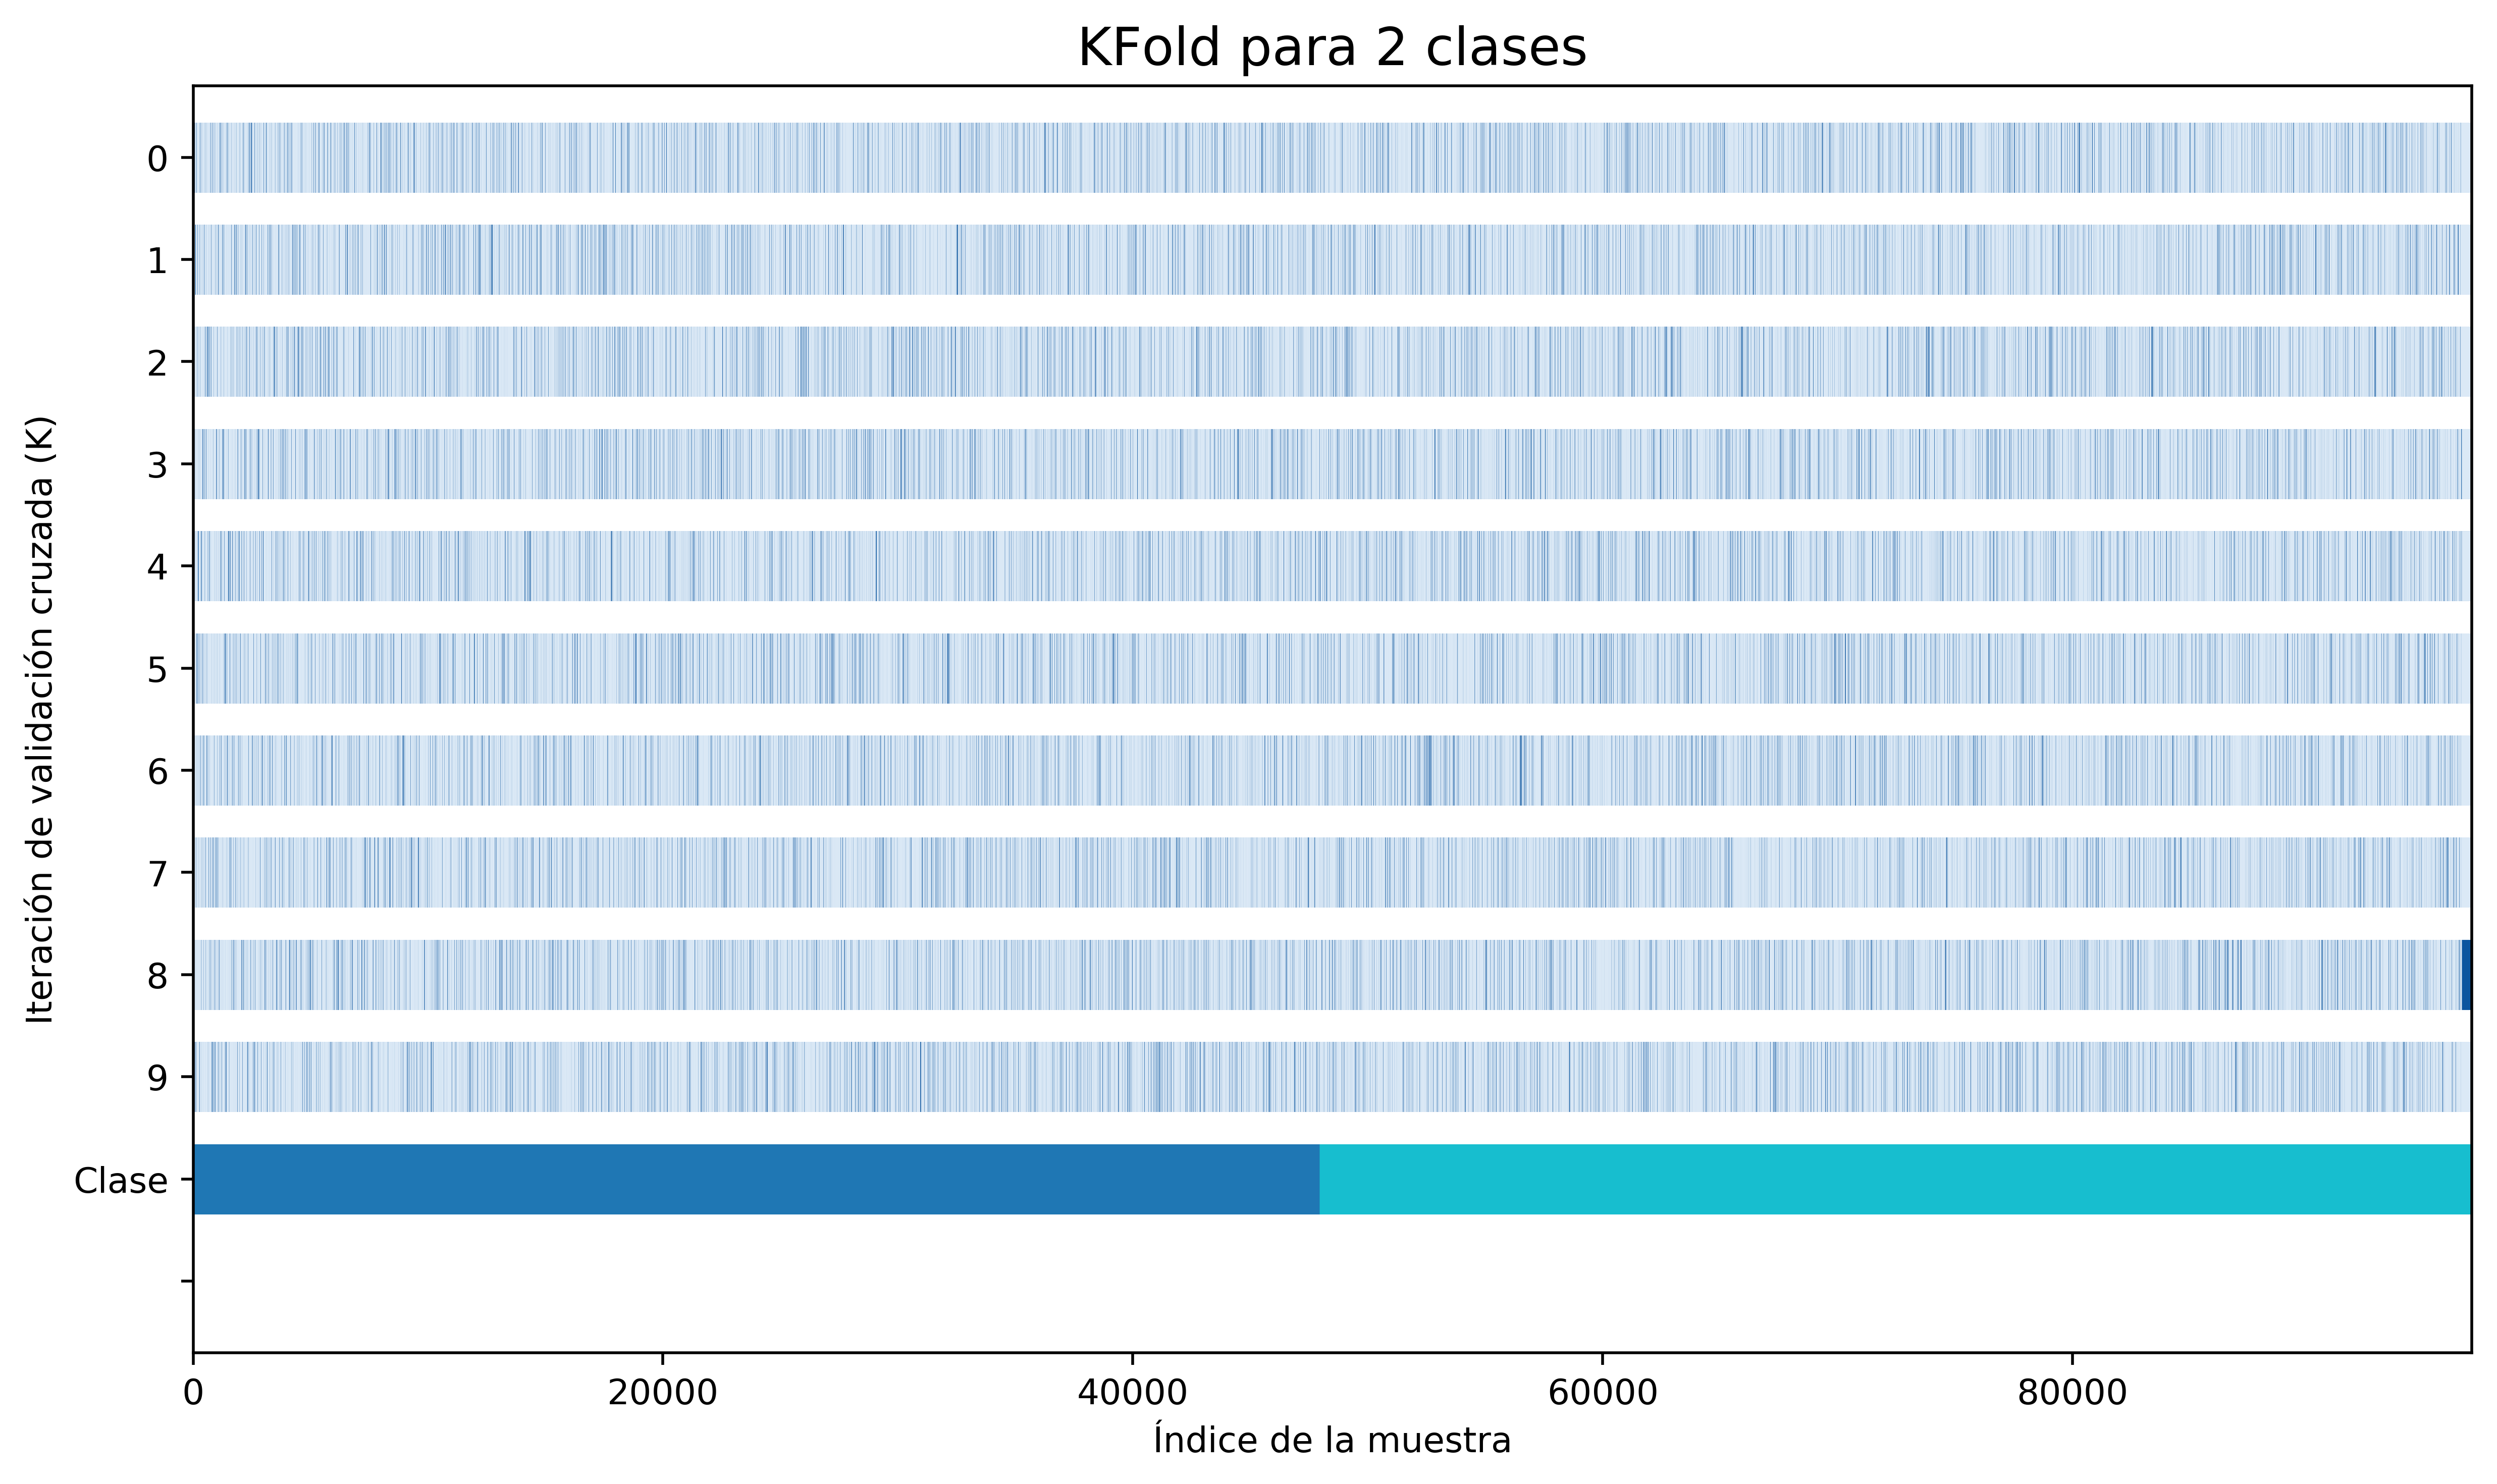
\includegraphics[width=0.9\textwidth]{capitulo_sdac/kfold_10_2.png}
    \caption{K-fold de 10 iteraciones binario}\label{fig:kfold}
\end{figure}

\subsubsection{Clasificación multi-clase}

La~\autoref{fig:kfold_7} muestra la validación cruzada\footnote{Debido a que se
usa la misma semilla para los experimentos, los números aleatorios generados son
bastante similares en los experimentos.} aplicada al problema de siete clases.
Existe discrepancia en la cantidad de elementos por cada una de las clases, es
decir, es un entrenamiento desbalanceado y procederemos a evaluar el impacto de
ello en el experimento. Este entrenamiento fue sumamente tardado: 44 horas, ya
que duplicamos el número de épocas de entrenamiento.

\begin{figure}[H]
    \centering
    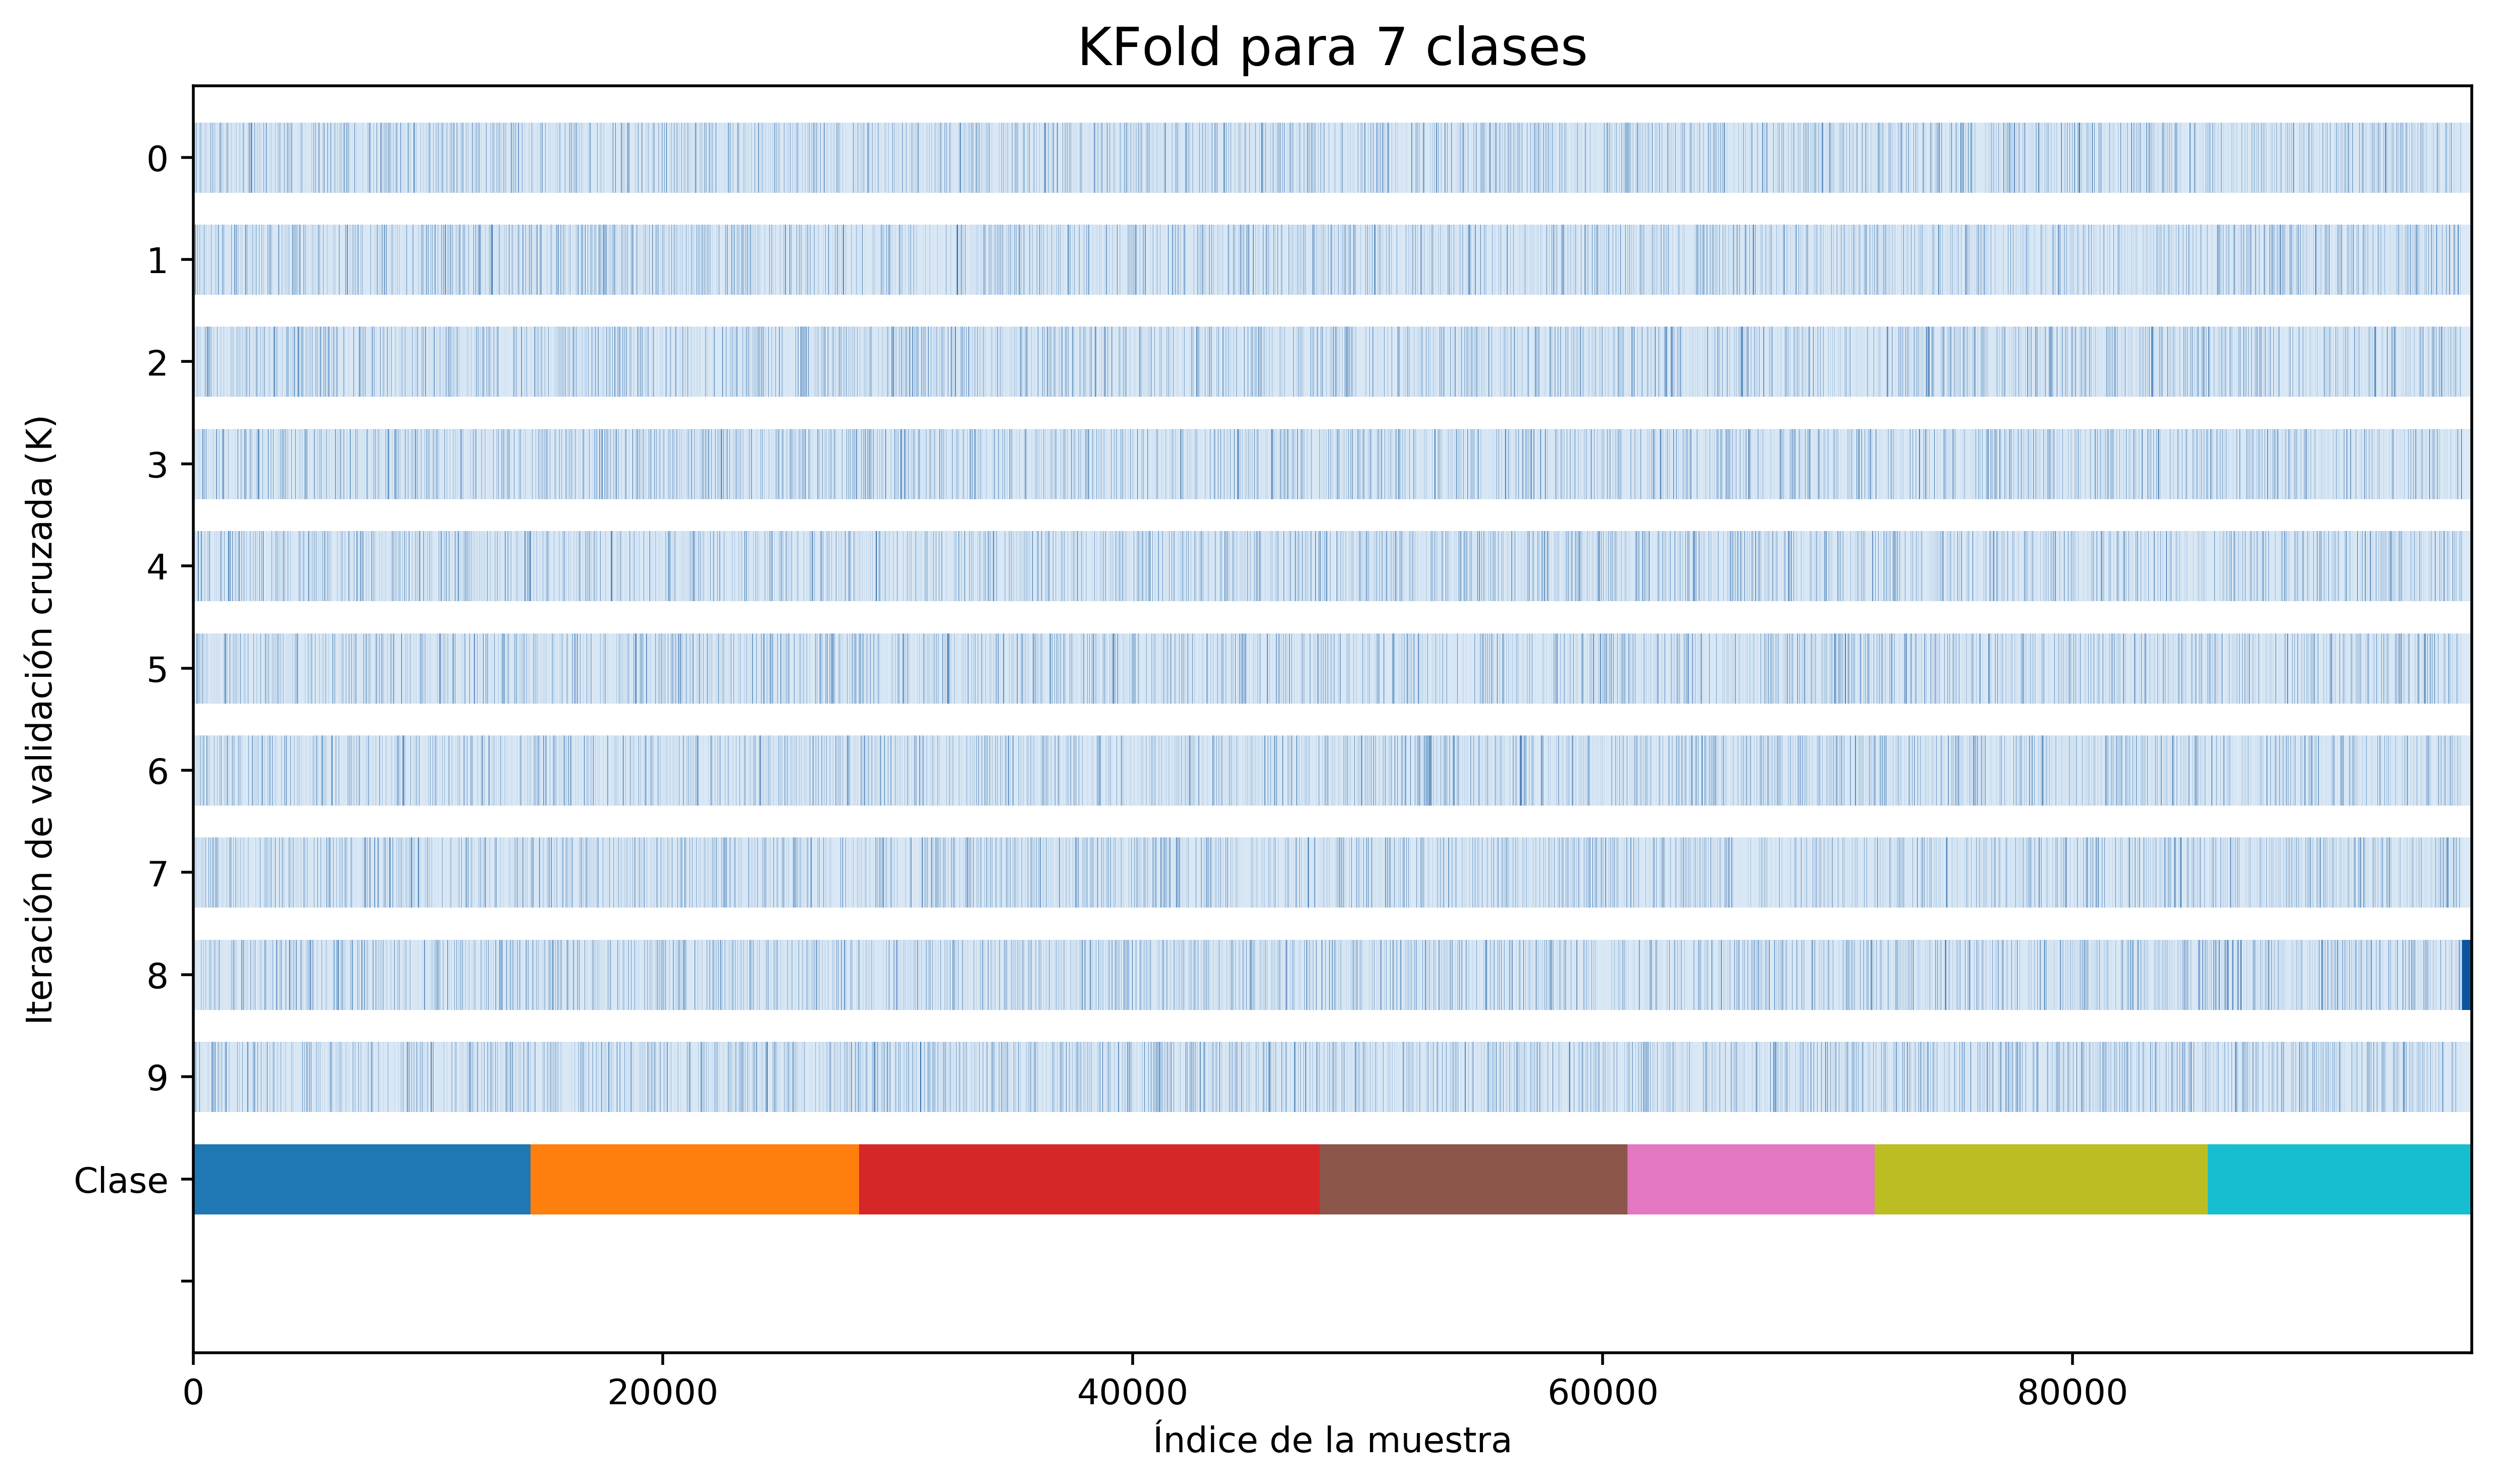
\includegraphics[width=0.9\textwidth]{capitulo_sdac/kfold_10_7.png}
    \caption{K-fold de 10 iteraciones multi-clase}\label{fig:kfold_7}
\end{figure}

\subsection{Elegir hiperparámetros}

Una correcta elección de hiperparámetros asegura que el modelo convergerá para
dar solución al problema. Si elegimos mal puede hacer que el algoritmo jamás
funcione o tenga un comportamiento errático. 

\begin{itemize}
    \item El tamaño de lote o \mintinline{latex}{BATCH_SIZE} se dejó como máximo
    en \(64\). Más grande hacía que el \hyperlink{abbr}{GPU} se quedara sin
    memoria antes de terminar.
    \item Las neuronas de la capa densa o totalmente conectada
    \mintinline{latex}{FC_LAYERS} se dejan en \(1024\) neuronas en comparación a
    las \(4096\) que tiene VGG original.
    \item Como optimizador \mintinline{latex}{OPT} se eligió Adam\footnote{Otros
    algoritmos pueden ser SGD y SGD con momento.} y este cuenta con solo un
    hiper-parámetro \mintinline{latex}{LR} que es la tasa de aprendizaje. Para
    \hyperlink{abbr}{TL} se prefieren tasas pequeñas.
    \item \mintinline{latex}{DROPOUT} define la probabilidad de apagar una
    neurona particular en las capas densas y generalmente se sitúa en \(50\%\).
\end{itemize}

\subsubsection{Clasificación binaria}

Los hiperparámetros usados para el entrenamiento del modelo se muestran a
continuación. La variable global \mintinline{latex}{KFOLD_SPLITS} determina la
cantidad de iteraciones en la validación cruzada, lo cual nos permite evaluar el
rendimiento del algoritmo con la mayor exactitud posible y con las mejores
prácticas estadísticas (\autoref{fig:hiper_dosclases}).

\begin{figure}[H]
    \centering
    \begin{minted}{python}
                        BATCH_SIZE = 64
                        FC_LAYERS = [1024, 1024]
                        LR = 0.00001
                        OPT = Adam(lr=LR)
                        EPOCHS = 30
                        DROPOUT = 0.5
                        KFOLD_SPLITS = 10
    \end{minted}
     \caption{Hiperparámetros para dos clases}\label{fig:hiper_dosclases}
\end{figure}

\subsubsection{Clasificación multi-clase}

A continuación se muestran los hiperparámetros utilizados, se incrementó la tasa
de aprendizaje y se duplicó el numero de épocas debido a la mayor complejidad
del problema  (\autoref{fig:hiper_sieteclases}), debido a esto el experimento
tardó el doble en completarse como era lógico:

\begin{figure}[H]
    \centering
\begin{minted}{python}
                        BATCH_SIZE = 64
                        FC_LAYERS = [1024, 1024]
                        LR = 0.0001
                        OPT = Adam(lr=LR)
                        EPOCHS = 60
                        DROPOUT = 0.5
                        KFOLD_SPLITS = 10
\end{minted}
\caption{Hiperparámetros para siete clases}\label{fig:hiper_sieteclases}
\end{figure}

\subsubsection{Segmentación semántica}

Los hiperparámetros usados en el experimentos son los siguientes, notar que el
optimizador usa los valores por defecto que recomienda \textbf{Keras}. Se redujo
\mintinline{latex}{BATCH_SIZE} a la mitad ya que en realidad estamos pasando dos
imágenes por cada iteración de entrenamiento en lugar de una
(\autoref{fig:hiper_segmentacion}). Para este experimento nos conformaremos con
solo cinco iteraciones ya que los previos tardaron mucho:

\begin{figure}[H]
    \centering
\begin{minted}{python}
                        BATCH_SIZE = 32
                        LR = 0.001
                        OPT = Adam(lr=LR)
                        EPOCHS = 50
                        DROPOUT = 0.5
                        KFOLD_SPLITS = 5
\end{minted}
\caption{Hiperparámetros para segmentación semántica}\label{fig:hiper_segmentacion}
\end{figure}

\subsection{Entrenar modelo}

Una vez encontrado el mejor modelo, procederemos a aplicar Fine-Tuning y la
optimización de hiperparámetros. La última capa del modelo pre-entrenado fue
removida y reemplazada por una capa densa totalmente conectada, para luego ser
entrenada en conjunto a toda la red. Convirtiendo un modelo general en un
predictor particular, capaz de clasificar células en distintas clases.

El ciclo de entrenamiento (\autoref{alg:entrenamiento}) es general para los tres
experimentos. Recibe como entrada una \hyperlink{abbr}{BD} representada por un
archivo \emph{.csv} cargado a memoria como DataFrame y como salida da el mejor
modelo. La variable \mintinline{latex}{results} es una lista que va a guardar el
rendimiento de cada modelo entrenado en cada iteración \mintinline{latex}{k =
5}. La función \mintinline{latex}{Kfold} divide los datos y devuelve
\mintinline{latex}{j, train, val} que son el índice de la iteración, los índices
de entrenamiento y los índices de validación. Se construye el modelo pasando los
hiperparámetros a la función \mintinline{latex}{build_model}. Se guarda el
resultado de ajustar el modelo por el número de épocas. El error de
generalización es el promedio del rendimiento de todos los resultados y se
escoge el mejor modelo con la función \mintinline{latex}{best_index} que
devuelve el índice del elemento más grande en la lista
\mintinline{latex}{results}.

\begin{algorithm}
    \SetAlgoLined{}
    \SetKwInOut{Input}{Input}\SetKwInOut{Output}{Output}
    \Input{Database}
    \Output{Best model}
    \(results \longleftarrow [ \cdots ]\)
    \BlankLine{}
    \(models \longleftarrow [ \cdots ]\)
    \BlankLine{}
    \(batch\_size \longleftarrow 128\)
    \BlankLine{}
    \(epochs \longleftarrow 50\)
    \BlankLine{}
    \(layers \longleftarrow [1024, 1024]\)
    \BlankLine{}
    \(opt \longleftarrow Adam\)
    \BlankLine{}
    \(lr \longleftarrow 1e-4\)
    \BlankLine{}
    \(dropout \longleftarrow [0.5, 0.5]\)
    \BlankLine{}
    \(k \longleftarrow 5\)
    \BlankLine{}
    \(\mathbb{D}  \longleftarrow database\)
    \BlankLine{}
    \For{\(j, train, val \in Kfold(splits=k, data=\mathbb{D})\)}{    
        \BlankLine{}
        \(model = build\_model(dropout, layers, opt(lr))\)
        \BlankLine{}
        \(result = model.fit(train, epochs)\)
        \BlankLine{}
        \(models[j] \longleftarrow model\)
        \(results[j] \longleftarrow result.evaluate(val)\)
    }
    \BlankLine{}
    \(generalization\_error \longleftarrow mean(results)\)
    \BlankLine{}
    \(best\_model\_idx \longleftarrow best\_index(results)\)
    \BlankLine{}
    \(best\_model = models[best\_model\_idx]\)
    \caption{Ciclo de entrenamiento}\label{alg:entrenamiento}
\end{algorithm}

Las tablas de rendimiento por época para los tres experimentos se pueden
encontrar en el \autoref{appendix:entrenamiento}.

\subsubsection{Clasificación binaria}

La~\autoref{tabla:rendimiento:final} nos muestra como se comportó el modelo
en las 30 épocas de entrenamiento tanto en entrenamiento como en validación. Es
clara la tendencia del algoritmo a mejorar con respeto a las épocas, aunque se
sigue notando cierta discrepancia entre los valores de validación y
entrenamiento, queremos que estos valores sean lo más cercanos posibles.

Los resultados de la validación cruzada se pueden observar el
la~\autoref{tabla:validacion}. La iteración con mejor rendimiento fue la número
6, alcanzando una exactitud del 99.91\%.

% Please add the following required packages to your document preamble:
% \usepackage{booktabs}
% \usepackage{graphicx}
\begin{table}[H]
    \centering
    \resizebox{0.4\textwidth}{!}{%
    \begin{tabular}{@{}lll@{}}
    \toprule
    fold & acc & loss \\ \midrule
    0 & 99.84536171 & 0.004982506 \\
    1 & 99.85566735 & 0.00357472 \\
    2 & 99.86597896 & 0.004019101 \\
    3 & 99.89690781 & 0.003187174 \\
    4 & 99.8865962 & 0.00304257 \\
    5 & 99.8865962 & 0.004015994 \\ \midrule
    6 & 99.91752505 & 0.002261744 \\ \midrule
    7 & 99.87629056 & 0.002811817 \\ 
    8 & 99.77319837 & 0.006879645 \\
    9 & 99.82474446 & 0.00390799 \\ \bottomrule
    \end{tabular}%
    }
    \caption{Resultados de la validación cruzada binaria}\label{tabla:validacion}
    \end{table}

La~\autoref{tabla:estadisticos} concluye el experimento, la exactitud final
alcanzada es el promedio de las iteraciones: \(99.86\% \pm 0.0412\). Un
rendimiento bastante aceptable, siendo el error de generalización del modelo un
total de \( 0.14\% \).

\begin{table}[H]
    \centering
    \resizebox{0.4\textwidth}{!}{%
    \begin{tabular}{@{}lll@{}}
    \toprule
     & acc & loss \\ \midrule
    count & 10 & 10 \\
    mean & 99.86288667 & 0.003868326 \\
    std & 0.041250406 & 0.001303197 \\
    min & 99.77319837 & 0.002261744 \\
    25\% & 99.84793812 & 0.003078721 \\
    50\% & 99.87113476 & 0.003741355 \\
    75\% & 99.8865962 & 0.004018324 \\
    max & 99.91752505 & 0.006879645 \\ \bottomrule
    \end{tabular}%
    }
    \caption{Estadísticos del experimento binario}\label{tabla:estadisticos}
    \end{table}

A continuación se mostrarán las métricas de la mejor iteración, que nos ofrecerá
información sobre el comportamiento del experimento y de su rendimiento. Las
métricas cuentan con su gráfica normal y una aplicando suavizado exponencial
para mejorar su interpretación.

La pérdida durante el entrenamiento y validación se muestran en
la~\autoref{fig:perdida_total}, donde la tendencia a disminuir es clara,
estabilizándose alrededor de la época número 15.

\begin{figure}[H]
    \centering
    \includegraphics[width=0.7\textwidth]{capitulo_sdac/reporte_2_class/loss.pdf}
    \caption{Pérdida binaria}\label{fig:perdida_total}
\end{figure}

La exactitud se estabiliza alrededor de la época 15 como se muestra en
la~\autoref{fig:precision_total}. Se detecta que tanto en la pérdida como en la
exactitud que ambas curvas se acercan la una a la otra, lo que nos dice que el
modelo está ajustado de manera excelente.

\begin{figure}[H]
    \centering
    \includegraphics[width=0.7\textwidth]{capitulo_sdac/reporte_2_class/acc.pdf}
    \caption{Precisión binaria}\label{fig:precision_total}
\end{figure}
    
\subsubsection{Clasificación multi-clase}

La~\autoref{tabla:rendimiento_7} nos permite ver que el algoritmo incrementa su
rendimiento al pasar las épocas, aunque cada vez se le hace más difícil mejorar
sus métricas. Quizás se puedan implementar acciones que optimicen los
hiperparámetros o inclusive técnicas de entrenamiento adaptativas o quizás
probar con otro optimizador.

Los resultados de la validación cruzada de 10 iteraciones para el experimento
multi-clase se ven en la~\autoref{tabla:validacion7}. La iteración con mejor
rendimiento fue la número 1, alcanzando una exactitud del 99.72\%. Se manifiesta
cierto fenómeno donde la pérdida de la iteración 0 es mejor que la 1. Esto puede
ser debido a fluctuaciones del generador de números aleatorios.

\begin{table}[H]
    \centering
    \resizebox{0.4\textwidth}{!}{%
    \begin{tabular}{@{}lll@{}}
    \toprule
    fold & acc & loss \\ \midrule
    0 & 99.69072342 & 0.009913217 \\ \midrule
    1 & 99.72165227 & 0.010205996 \\ \midrule
    2 & 99.59793687 & 0.013710575 \\
    3 & 99.49484468 & 0.014681551 \\
    4 & 99.49484468 & 0.016252176 \\
    5 & 99.60824847 & 0.0124342 \\
    6 & 99.60824847 & 0.011963185 \\
    7 & 99.57731962 & 0.014334826 \\
    8 & 99.46391582 & 0.016523478 \\
    9 & 99.62886572 & 0.013009808 \\ \bottomrule
    \end{tabular}%
    }
    \caption{Resultados de la validación cruzada multi-clase}\label{tabla:validacion7}
    \end{table}

La~\autoref{tabla:estadisticos7} concluye el experimento, la exactitud final
alcanzada es el promedio de las iteraciones: \(99.58\% \pm 0.084\). Podemos ver
que tanto la especificidad como la sensibilidad tienen una desviación estándar
mayor que la exactitud, debido a la forma en que se calculan estas métricas. El
error de generalización total del modelo es de 0.42\%.

\begin{table}[H]
    \centering
    \resizebox{0.4\textwidth}{!}{%
    \begin{tabular}{@{}lll@{}}
    \toprule
     & acc & loss \\ \midrule
    count & 10 & 10 \\
    mean & 99.58866 & 0.013302901 \\
    std & 0.084239213 & 0.002258767 \\
    min & 99.46391582 & 0.009913217 \\
    25\% & 99.51546341 & 0.012080938 \\
    50\% & 99.60309267 & 0.013360192 \\
    75\% & 99.62371141 & 0.01459487 \\
    max & 99.72165227 & 0.016523478 \\ \bottomrule
    \end{tabular}%
    }
    \caption{Estadísticos del experimento multi-clase}\label{tabla:estadisticos7}
    \end{table}

La pérdida cayó abruptamente antes de las 10 épocas, después de las cuales se
estabilizó alcanzando cierto límite asintótico; Cuando se analiza la diferencia
entre la pérdida en entrenamiento y validación, estas se encuentran muy cercanas
y casi iguales lo cual es ideal, quiere decir que nuestro modelo puede capturar
muy bien las complejidades de la clasificación citológica multi-clase
(\autoref{fig:perdida_total_7}).

\begin{figure}[H]
    \centering
    \includegraphics[width=0.7\textwidth]{capitulo_sdac/reporte_7_class/loss.pdf}
    \caption{Pérdida con 7 clases}\label{fig:perdida_total_7}
\end{figure}

La exactitud del experimento multi-clase se comporta muy similar al del
experimento binario (\autoref{fig:precision_total_7}). Hay una mínima brecha
entre la métrica en entrenamiento y en validación probablemente se deba al
fenómeno de~\emph{underfitting}. Esto se podría solucionar reduciendo el
\mintinline{latex}{DROPOUT} o incrementando la complejidad del modelo, aunque la
diferencia es tan poca que puede no ser significativa.

\begin{figure}[H]
    \centering
    \includegraphics[width=0.7\textwidth]{capitulo_sdac/reporte_7_class/acc.pdf}
    \caption{Exactitud con 7 clases}\label{fig:precision_total_7}
\end{figure}


\subsubsection{Segmentación semántica}

En la segmentación semántica substituiremos las métricas de clasificación por la
Intersección sobre Union y la función de pérdida por el coeficiente de Dice, ya
que son las indicadas para arquitectura usada en este caso.

Los resultados de la validación cruzada para segmentación, con cinco
iteraciones, se compilan en la~\autoref{tabla:rendseg}, mientras que el resumen
y los estadísticos están en la~\autoref{tabla:estadisticosseg}. Claramente es la
primera iteración la que alcanzó los mejores resultados. Esta pérdida puede
tener valores negativos en comparación a la usada en las arquitecturas
anteriores. Si bien la exactitud es la métrica más alta, en este caso, la
correcta es IoU con un rendimiento total de 88.19\%.

\begin{table}[H]
    \centering
    \resizebox{0.5\textwidth}{!}{%
    \begin{tabular}{@{}llll@{}}
    \toprule
    fold & accuracy & loss & iou \\ \midrule
    0 & 91.0180247 & -0.896642793 & 0.884503568 \\ \midrule
    1 & 89.86388168 & -0.917515639 & 0.888006022 \\
    2 & 89.99839323 & -0.911953644 & 0.885471006 \\
    3 & 89.79965767 & -0.900890709 & 0.866708054 \\
    4 & 90.36797129 & -0.911352285 & 0.885264954 \\ \bottomrule
    \end{tabular}%
    }
    \caption{Rendimiento de la validación cruzada de segmentación}\label{tabla:rendseg}
    \end{table}

\begin{table}[H]
    \centering
    \resizebox{0.6\textwidth}{!}{%
    \begin{tabular}{@{}llll@{}}
    \toprule
    & accuracy & loss & iou \\ \midrule
    Número & 5 & 5 & 5 \\
    Media & 90.20958571 & -0.907671014 & 0.881990721 \\
    Desviación & 0.502696262 & 0.008608186 & 0.008644234 \\
    Mínimo & 89.79965767 & -0.917515639 & 0.866708054 \\
    25\% & 89.86388168 & -0.911953644 & 0.884503568 \\
    50\% & 89.99839323 & -0.911352285 & 0.885264954 \\
    75\% & 90.36797129 & -0.900890709 & 0.885471006 \\
    Máximo & 91.0180247 & -0.896642793 & 0.888006022 \\ \bottomrule
    \end{tabular}%
    } 
    \caption{Estadísticos del experimento}\label{tabla:estadisticosseg}
    \end{table}

La~\autoref{fig:perdida_seg} muestra los resultados de la pérdida en
entrenamiento y validación. Se pueden observar fluctuaciones considerables en
validación con una clara tendencia a estabilizarse conforme pasan las épocas de
entrenamiento.

\begin{figure}[H]
    \centering
    \includegraphics[width=0.7\textwidth]{capitulo_sdac/perdida_2.pdf}
    \caption{Gráfico de pérdida, se nota fluctuación en validación}\label{fig:perdida_seg}

\end{figure}

A continuación vemos (\autoref{fig:acc_total_seg}) la \emph{Intersection over
Union} en las dos fases. Se manifiesta una excelente curva que aumenta
constantemente en función de las épocas, reduciendo su incremento en cada
iteración pero siempre aumentando, igualmente, las dos curvas se mantienen muy
próximas entre si.

\begin{figure}[H]
    \centering
    \includegraphics[width=0.7\textwidth]{capitulo_sdac/exactitud_2.pdf}
    \caption{Gráfico de Intersección sobre Unión}\label{fig:acc_total_seg}

\end{figure}

\subsection{Evaluar modelo}

Para evaluar el modelo, primeramente haremos un análisis comparativo de las
métricas en validación y entrenamiento. En los problemas de clasificación, es
común realizar una gráfica conocida como Matriz de Confusión que nos permite ver
fácilmente la cantidad de elementos clasificados correcta o incorrectamente.
Aplicaremos un total de 22 métricas de evaluación para estimar, con la mayor
certeza posible, el rendimiento del modelo ya que su aplicación final será para
diagnóstico de cáncer.

Por último, tomaremos un muestreo de aquellas células que fueron mal
clasificadas, para poder observar las características morfológicas y apreciar
empíricamente los errores.

\subsubsection{Clasificación binaria}

Para determinar como difieren los valores de entrenamiento y validación, se
realizó una gráfica de caja con las métricas y la pérdida. La variabilidad
individual de estas métricas se muestra en la~\autoref{fig:caja_total2}. Se
aprecia que en la fase de entrenamiento, las métricas tienen una variabilidad
mayor, esto es debido a que la validación se hace siempre una época después que
el entrenamiento, por lo que esta se realiza con los pesos ya ajustados por la
función de pérdida, reduciendo su error total.

\begin{figure}[H]
    \centering
    \begin{subfigure}[b]{0.6\textwidth}
        \centering
        \includegraphics[width=1\textwidth]{capitulo_sdac/reporte_2_class/box_acc.pdf}
        \caption{Gráfico de caja de métricas}\label{fig:caja_acc2} 
    \end{subfigure}

    \begin{subfigure}[b]{0.6\textwidth}
        \centering
        \includegraphics[width=1\textwidth]{capitulo_sdac/reporte_2_class/box_loss.pdf}
        \caption{Gráfico de caja de pérdida}\label{fig:caja_loss2}
    \end{subfigure}
    \caption{Gráficos de caja binarios}\label{fig:caja_total2}
\end{figure}

La~\autoref{fig:caja_total} nos muestra la comparación de la variabilidad entre
la pérdida y la exactitud en validación, donde comprobamos efectivamente que su
variabilidad se reduce conforme pasan las épocas de entrenamiento y que el
modelo puede generalizar correctamente. Como ya sabemos, entre más cerca estén
las métricas, mejor.

\begin{figure}[H]
    \centering
    \begin{subfigure}[b]{0.6\textwidth}
        \centering
        \includegraphics[width=1\textwidth]{capitulo_sdac/reporte_2_class/variabilidad_acc.pdf}
        \caption{Variación en la exactitud}\label{fig:caja_acc} 
    \end{subfigure}

    \begin{subfigure}[b]{0.6\textwidth}
        \centering
        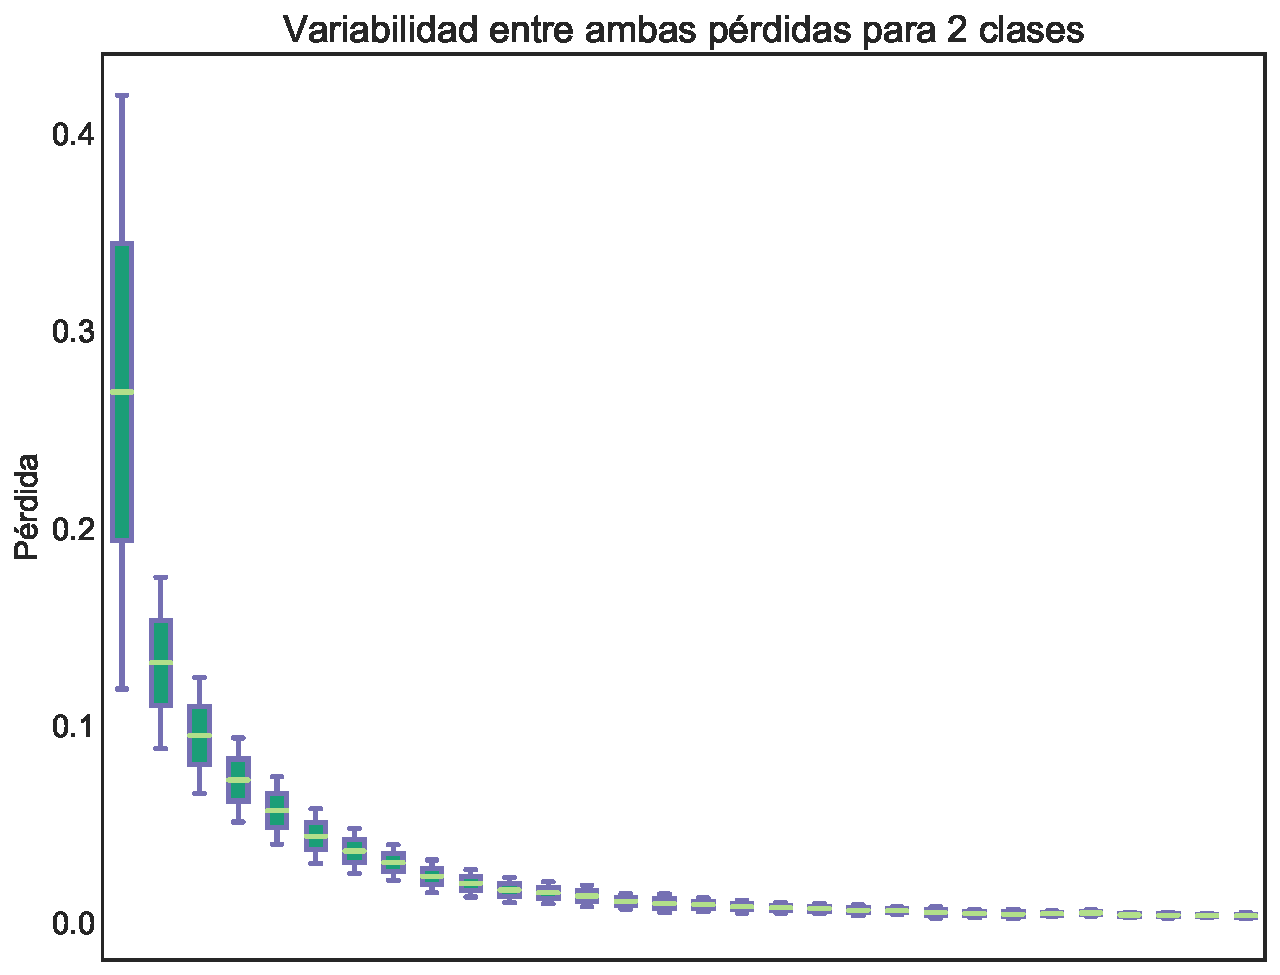
\includegraphics[width=1\textwidth]{capitulo_sdac/reporte_2_class/variabilidad_loss.pdf}
        \caption{Variación en la pérdida}\label{fig:caja_loss}
    \end{subfigure}
    \caption{Gráfica de caja de la variación binaria}\label{fig:caja_total}
\end{figure}

La~\autoref{tabla:reporte_2} nos muestra el reporte que evalúa un algoritmo de
clasificación, condensando la información básica por cada clase. Cabe notar que
los falsos positivos (FP) y falsos negativos (FN) son muy pocos comparados con
los datos utilizados para evaluar (POP). Las clases están desbalanceadas pero su
diferencia es una cantidad negligible. 

\begin{table}[H]
    \centering
    \resizebox{0.3\textwidth}{!}{%
    \begin{tabular}{@{}lll@{}}
    \toprule
    Class & anormal & normal \\ \midrule
    TP & 4899 & 4793 \\
    TN & 4793 & 4899 \\
    FP & 1 & 7 \\
    FN & 7 & 1 \\
    P & 4906 & 4794 \\
    N & 4794 & 4906 \\
    POP & 9700 & 9700 \\ \bottomrule
    \end{tabular}%
    }
    \caption{Reporte de clasificación binario}\label{tabla:reporte_2}
    \end{table}

La~\autoref{fig:matrices} nos muestra las matrices de confusión; la matriz
normalizada no se aprecia bien por el redondeo y se puede interpretar que el
sistema tiene un poder de clasificación perfecto, pero podemos ver en la matriz
no normalizada que un total de 8 elementos fueron mal clasificados, un ejemplo
normal clasificado como anormal y siete anormales clasificados como normales,
esto puede suponer un problema ya que es peligroso diagnosticar la ausencia de
lesión citológica cuando si está presente.

\begin{figure}[H]
    \centering
    \begin{subfigure}[b]{0.6\textwidth}
        \centering 
        \includegraphics[width=1\linewidth]{capitulo_sdac/reporte_2_class/matriz.pdf}
        \caption{Matriz de confusión normalizada}\label{fig:matriz_norm}
        \end{subfigure}
    \begin{subfigure}[b]{0.6\textwidth}
        \centering 
        \includegraphics[width=1\linewidth]{capitulo_sdac/reporte_2_class/matriz_norm.pdf}
        \caption{Matriz de confusión sin normalizar}\label{fig:matriz_sin}
    \end{subfigure}%
        \caption{Matrices de confusión}\label{fig:matrices}
\end{figure}
    
La~\autoref{tabla:reporte_completo_2} nos condensa todas las métricas utilizadas
para la evaluación del problema de clasificación de imágenes de células en dos
clases: anormal y normal. El rendimiento del modelo es bastante bueno y que la
elección de arquitectura fue correcta. Lo cual se probará con mayor atención en
el problema de siete clases. 

% Please add the following required packages to your document preamble:
% \usepackage{booktabs}
% \usepackage{graphicx}
\begin{table}[H]
    \centering
    \resizebox{0.3\textwidth}{!}{%
    \begin{tabular}{@{}lll@{}}
    \toprule
    Class & anormal & normal \\ \midrule
    TPR & 0.99857 & 0.99979 \\
    TNR & 0.99979 & 0.99857 \\
    PPV & 0.9998 & 0.99854 \\
    NPV & 0.99854 & 0.9998 \\
    FNR & 0.00143 & 0.00021 \\
    FPR & 0.00021 & 0.00143 \\
    FDR & 0.0002 & 0.00146 \\
    FOR & 0.00146 & 0.0002 \\
    ACC & 0.99918 & 0.99918 \\
    F1 & 0.99918 & 0.99917 \\
    BM & 0.99836 & 0.99836 \\
    PRE & 0.50577 & 0.49423 \\
    J & 0.99837 & 0.99833 \\
    CEN & 0.00881 & 0.00898 \\
    MCEN & 0.01598 & 0.01628 \\
    AUC & 0.99918 & 0.99918 \\ \bottomrule
    \end{tabular}%
    }
    \caption{Métricas de clasificación binaria}\label{tabla:reporte_completo_2}
    \end{table}

La \autoref{fig:reporte_2_0} nos muestra una mapa de calor que muestra las
métricas que deben ser 0 al evaluar el modelo. Podemos ver que, si bien no es
justamente 0 el valor mínimo, el rango de variación mostrado por la barra es muy
reducido, siendo la peor métrica MCEN y está solamente 0.015 arriba del óptimo.

\begin{figure}[H]
    \centering
    \includegraphics[width=0.4\textwidth,keepaspectratio]{capitulo_sdac/reporte_2_class/reporte_cero.pdf}
    \caption{Reporte de clasificación binario para métricas que deben tender a 0}\label{fig:reporte_2_0}
\end{figure}

Las métricas que deben de tender a 1 se muestran en la
\autoref{fig:reporte_2_1}. La variación entre el máximo y el mínimo es de 0.006. Se observa
un excelente rendimiento en estas métricas, todas arriba de 0.997.

\begin{figure}[H]
    \centering
    \includegraphics[width=0.4\textwidth,keepaspectratio]{capitulo_sdac/reporte_2_class/reporte_uno.pdf}
    \caption{Reporte de clasificación binario para métricas que deben tender a 1}\label{fig:reporte_2_1}
\end{figure}

La \autoref{fig:roc_auc} nos muestra la curva Receiver Operating Characteristic
y su métrica derivada, el área bajo su curva o AUC. Como podemos ver, la tasa de
falsos positivos y falsos negativos es bastante baja, es por ello que el AUC se
aproxima a uno.

\begin{figure}[H]
    \centering
    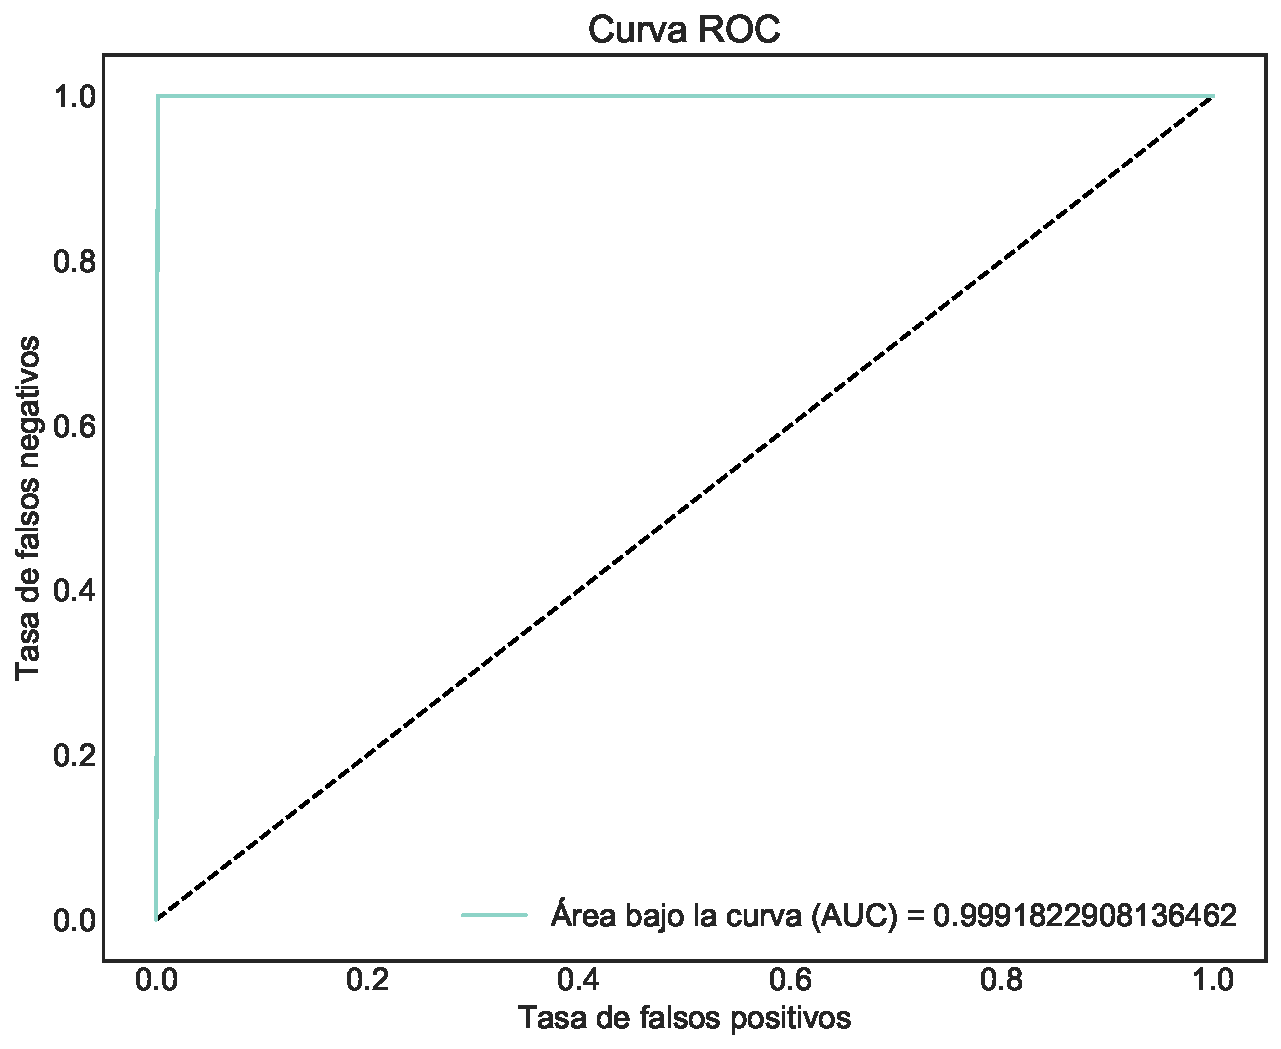
\includegraphics[width=0.7\textwidth]{capitulo_sdac/reporte_2_class/roc.pdf}
    \caption{Curva Receiver Operating Characteristic (ROC) y el Área bajo la curva (AUC)}\label{fig:roc_auc}
\end{figure}

Se muestra en la~\autoref{tabla:metricas_diag_2} el reporte de métricas
especiales utilizadas para sistemas de diagnóstico. PLR tiene mejor
representación en la clase anormal, probablemente debido a que contiene más
variación entre sus elementos ya que en realidad son siete clases en una
mientras que normal son tres en una. DOR implica que la prueba es igualmente
efectiva en ambas clases mientras que un DP arriba de tres se considera bueno.

\begin{table}[H]
    \centering
    \resizebox{0.35\textwidth}{!}{%
    \begin{tabular}{@{}lll@{}}
    \toprule
    Class & anormal & normal \\ \midrule
    PLR & 4787.1598 & 700.71095 \\
    NLR & 0.00143 & 0.00021 \\
    DOR & 3354415.286 & 3354415.286 \\
    DP & 3.59776 & 3.59776 \\
    IS & 0.98314 & 1.01465 \\ \bottomrule
    \end{tabular}%
    }
    \caption{Métricas para diagnóstico binario}\label{tabla:metricas_diag_2}
    \end{table}

De las 8 imágenes clasificadas incorrectamente, se tomaron cuatro muestras.
Cinco para aquellas células clasificadas incorrectamente como normales y cinco
para las clasificadas como anormales. Podemos ver en
la~\autoref{fig:muestreo_error_2}, que probablemente lo que incide en la mala
clasificación es la calidad de la imagen. Las células incorrectamente
clasificadas como normales son aquellas que tienen muestran una morfología
nuclear uniforme y pareja, en contraste con otras células cancerígenas. Las
células normales clasificadas como anormales, pertenecen todas a la clase
\emph{normal\_columnar}, ya que son las que tienen un núcleo más grande y este,
como se estipuló en los supuestos, es lo que determina la clase de una célula.

\begin{figure}[H]
    \centering
    \includegraphics[width=0.6\textwidth,keepaspectratio]{capitulo_sdac/reporte_2_class/muestras_erroneas.pdf}
    \caption{Muestreo de pruebas mal clasificadas binarias}\label{fig:muestreo_error_2}
\end{figure}


\subsubsection{Clasificación multi-clase}

La~\autoref{fig:caja_total7} muestra que en el experimento multi-clase, las
métricas de evaluación y entrenamiento varían más que en el experimento
anterior, como se puede observar en la amplitud de la gráfica de caja.
Probablemente se deba a que es un problema más complejo y con más clases.
También puede incidir en esto la decisión de hiperparámetros.

\begin{figure}[H]
    \centering
    \begin{subfigure}[b]{0.6\textwidth}
        \centering
        \includegraphics[width=1\textwidth]{capitulo_sdac/reporte_7_class/box_acc.pdf}
        \caption{Gráfico de caja de métricas}\label{fig:caja_acc7} 
    \end{subfigure}

    \begin{subfigure}[b]{0.6\textwidth}
        \centering
        \includegraphics[width=1\textwidth]{capitulo_sdac/reporte_7_class/box_loss.pdf}
        \caption{Gráfico de caja de pérdida}\label{fig:caja_loss7}
    \end{subfigure}
    \caption{Gráficos de caja multi-clase}\label{fig:caja_total7}
\end{figure}


Es en la comparativa de la variabilidad entre ambas métricas donde realmente nos
damos cuenta que (\autoref{fig:caja_total_7}) el modelo tiene más problemas que
el anterior en generalizar. La reducción entre la diferencia entre validación y
entrenamiento es mucho menor en cada época, decreciendo lenta pero segura para
converger a un mínimo.

\begin{figure}[H]
    \centering
    \begin{subfigure}[b]{0.6\textwidth}
        \centering
        \includegraphics[width=1\textwidth]{capitulo_sdac/reporte_7_class/variabilidad_acc.pdf}
        \caption{Variación en la exactitud multi-clase}\label{fig:caja_acc_7} 
    \end{subfigure}

    \begin{subfigure}[b]{0.6\textwidth}
        \centering
        \includegraphics[width=1\textwidth]{capitulo_sdac/reporte_7_class/variabilidad_acc.pdf}
        \caption{Variación en la pérdida multi-clase}\label{fig:caja_loss_7}
    \end{subfigure}
    \caption{Gráfica de caja de la variación multi-clase}\label{fig:caja_total_7}
\end{figure}

En la~\autoref{tabla:reporte_class_7} vemos que el total de elementos utilizados
para la evaluación fue de 9700. Las células normales tienen a ser mejor clasificadas que
las anormales, esto se puede deber al desbalance que existe en la base de datos. De las
células normales la clase~\emph{normal\_columnar} es la que más errores presenta, lo cual
concuerda con los resultados de la clasificación binaria debido a su morfología.

\begin{table}[H]
    \centering
    \resizebox{0.5\textwidth}{!}{%
    \begin{tabular}{@{}llllllll@{}}
    Class & \rot{\shortstack[l]{carcinoma\_in\_situ}} & \rot{\shortstack[l]{light\_dysplastic}} & \rot{\shortstack[l]{moderate\_dysplastic}} & \rot{\shortstack[l]{normal\_columnar}} &\rot{\shortstack[l]{normal\_intermediate}} & \rot{\shortstack[l]{normal\_superficiel}} & \rot{\shortstack[l]{severe\_dysplastic}} \\ \midrule
    TP & 1115 & 1247 & 1039 & 1965 & 1392 & 1503 & 1412 \\
    TN & 8566 & 8451 & 8649 & 7731 & 8308 & 8197 & 8271 \\
    FP & 14 & 2 & 4 & 2 & 0 & 0 & 5 \\
    FN & 5 & 0 & 8 & 2 & 0 & 0 & 12 \\
    P & 1120 & 1247 & 1047 & 1967 & 1392 & 1503 & 1424 \\
    N & 8580 & 8453 & 8653 & 7733 & 8308 & 8197 & 8276 \\
    POP & 9700 & 9700 & 9700 & 9700 & 9700 & 9700 & 9700 \\ \bottomrule
    \end{tabular}%
    }
    \caption{Reporte de clasificación multi-clase}\label{tabla:reporte_class_7}
    \end{table}

% \begin{table}[H]
%     \centering
%     \resizebox{\textwidth}{!}{%
%     \begin{tabular}{@{}llllllll@{}}
%     \toprule
%     Class & carcinoma\_in\_situ & light\_dysplastic & moderate\_dysplastic & normal\_columnar & normal\_intermediate & normal\_superficiel & severe\_dysplastic \\ \midrule
%     TP & 1115 & 1247 & 1039 & 1965 & 1392 & 1503 & 1412 \\
%     TN & 8566 & 8451 & 8649 & 7731 & 8308 & 8197 & 8271 \\
%     FP & 14 & 2 & 4 & 2 & 0 & 0 & 5 \\
%     FN & 5 & 0 & 8 & 2 & 0 & 0 & 12 \\
%     P & 1120 & 1247 & 1047 & 1967 & 1392 & 1503 & 1424 \\
%     N & 8580 & 8453 & 8653 & 7733 & 8308 & 8197 & 8276 \\
%     POP & 9700 & 9700 & 9700 & 9700 & 9700 & 9700 & 9700 \\ \bottomrule
%     \end{tabular}%
%     }
%     \caption{Reporte de clasificación multi-clase}
%     \label{tabla:reporte_class_}
%     \end{table}

Las matriz de confusión normalizada nos muestra una muy buena información sobre
el buen rendimiento del modelo. Esto lo podemos notar en
la~\autoref{fig:matriz_norm_7}. Observamos la diagonal muy bien marcada sin
rastros de azul en otras partes de la gráfica.

\begin{figure}[H]
    \centering
    \includegraphics[width=0.7\textwidth]{capitulo_sdac/reporte_7_class/matriz_norm.pdf}
    \caption{Matriz de confusión normalizada multi-clase}\label{fig:matriz_norm_7}
\end{figure}

La matriz de confusión sin normalizar (\autoref{fig:matriz_sin_7}) nos muestra
con mayor claridad los errores de clasificación. La diferencia en tonalidad de
azul en la diagonal de la matriz se debe a que cada clase tiene diferente número
de elementos. El modelo tiende a confundir más las clases
\emph{carcinoma\_in\_situ} y \emph{severe\_dysplastic}, puesto que una es una
etapa previa a la otra, no es tanto problema durante el diagnóstico médico.

\begin{figure}[H]
    \centering
    \includegraphics[width=0.7\textwidth]{capitulo_sdac/reporte_7_class/matriz.pdf}
    \caption{Matriz de confusión sin normalizar con 7 clases}\label{fig:matriz_sin_7}
\end{figure}

La~\autoref{tabla:metricas_class_7} resume todas las métricas utilizadas para la
evaluación posterior del modelo. Son las clases \emph{normal\_intermediate} y
\emph{normal\_superficiel} las mejor clasificadas, teniendo un rendimiento
perfecto, esto es obvio debido a sus características morfológicas con su núcleo
pequeño y bien diferenciado. 

% Please add the following required packages to your document preamble:
% \usepackage{graphicx}
\begin{table}[H]
    \centering
    \resizebox{0.7\textwidth}{!}{%
    \begin{tabular}{llllllll}
    Class & \rot{\shortstack[l]{carcinoma\_in\_situ}} & \rot{\shortstack[l]{light\_dysplastic}} & \rot{\shortstack[l]{moderate\_dysplastic}} & \rot{\shortstack[l]{normal\_columnar}} &\rot{\shortstack[l]{normal\_intermediate}} & \rot{\shortstack[l]{normal\_superficiel}} & \rot{\shortstack[l]{severe\_dysplastic}} \\ \midrule
    TPR & 0.99554 & 1 & 0.99236 & 0.99898 & 1 & 1 & 0.99157 \\
    TNR & 0.99837 & 0.99976 & 0.99954 & 0.99974 & 1 & 1 & 0.9994 \\
    PPV & 0.9876 & 0.9984 & 0.99616 & 0.99898 & 1 & 1 & 0.99647 \\
    NPV & 0.99942 & 1 & 0.99908 & 0.99974 & 1 & 1 & 0.99855 \\
    FNR & 0.00446 & 0 & 0.00764 & 0.00102 & 0 & 0 & 0.00843 \\
    FPR & 0.00163 & 0.00024 & 0.00046 & 0.00026 & 0 & 0 & 0.0006 \\
    FDR & 0.0124 & 0.0016 & 0.00384 & 0.00102 & 0 & 0 & 0.00353 \\
    FOR & 0.00058 & 0 & 0.00092 & 0.00026 & 0 & 0 & 0.00145 \\
    ACC & 0.99804 & 0.99979 & 0.99876 & 0.99959 & 1 & 1 & 0.99825 \\
    F1 & 0.99155 & 0.9992 & 0.99426 & 0.99898 & 1 & 1 & 0.99402 \\
    BM & 0.9939 & 0.99976 & 0.9919 & 0.99872 & 1 & 1 & 0.99097 \\
    PRE & 0.11546 & 0.12856 & 0.10794 & 0.20278 & 0.14351 & 0.15495 & 0.1468 \\
    J & 0.98325 & 0.9984 & 0.98858 & 0.99797 & 1 & 1 & 0.9881 \\
    CEN & 0.02137 & 0.00252 & 0.01586 & 0.00325 & 0 & 0 & 0.01549 \\
    MCEN & 0.03776 & 0.00459 & 0.02838 & 0.00592 & 0 & 0 & 0.0275 \\
    AUC & 0.99695 & 0.99988 & 0.99595 & 0.99936 & 1 & 1 & 0.99548
    \end{tabular}%
    }
    \caption{Métricas de clasificación multi-clase}\label{tabla:metricas_class_7}
    \end{table}

La~\autoref{fig:reporte_7_0} y~\autoref{fig:reporte_7_1} nos muestran, en un
mapa de calor las técnicas cuyo valor óptimo debe tender a 0 y a 1
respectivamente. Las métricas CEN, MCEN son las que peor evalúan al algoritmo,
sin embargo, la divergencia del óptimo es muy poca. Siendo la clase
\emph{severe\_dysplastic} la que peor rendimiento tiene, que es confundida por
cáncer habitualmente.

\begin{figure}[H]
    \centering
    \includegraphics[width=0.7\textwidth,keepaspectratio]{capitulo_sdac/reporte_7_class/reporte_cero.pdf}
    \caption{Reporte de clasificación multi-clase para métricas que deben tender a 0}\label{fig:reporte_7_0}
\end{figure}

\begin{figure}[H]
    \centering
    \includegraphics[width=0.7\textwidth,keepaspectratio]{capitulo_sdac/reporte_7_class/reporte_uno.pdf}
    \caption{Reporte de clasificación multi-clase para métricas que deben tender a 1}\label{fig:reporte_7_1}
\end{figure}

La curva ROC y AUC generalmente se utilizan para problemas de clasificación
binarios, se pudo adaptar al problema multi-clase  realizando una cruza todos
contra todos de los valores de validación podemos generar las métricas y grafica
multi-clase. El macro-promedio computa la métrica independiente para cada clase
y luego toma el promedio; mientras que el micro-promedio agrega las
contribuciones de todas las clases y computa el promedio, este ultimo es
significativo para pruebas multi-clase debido a que toma en cuenta la falta de
balance entre las clases (\autoref{fig:roc_multi}).

\begin{figure}[H]
    \centering
    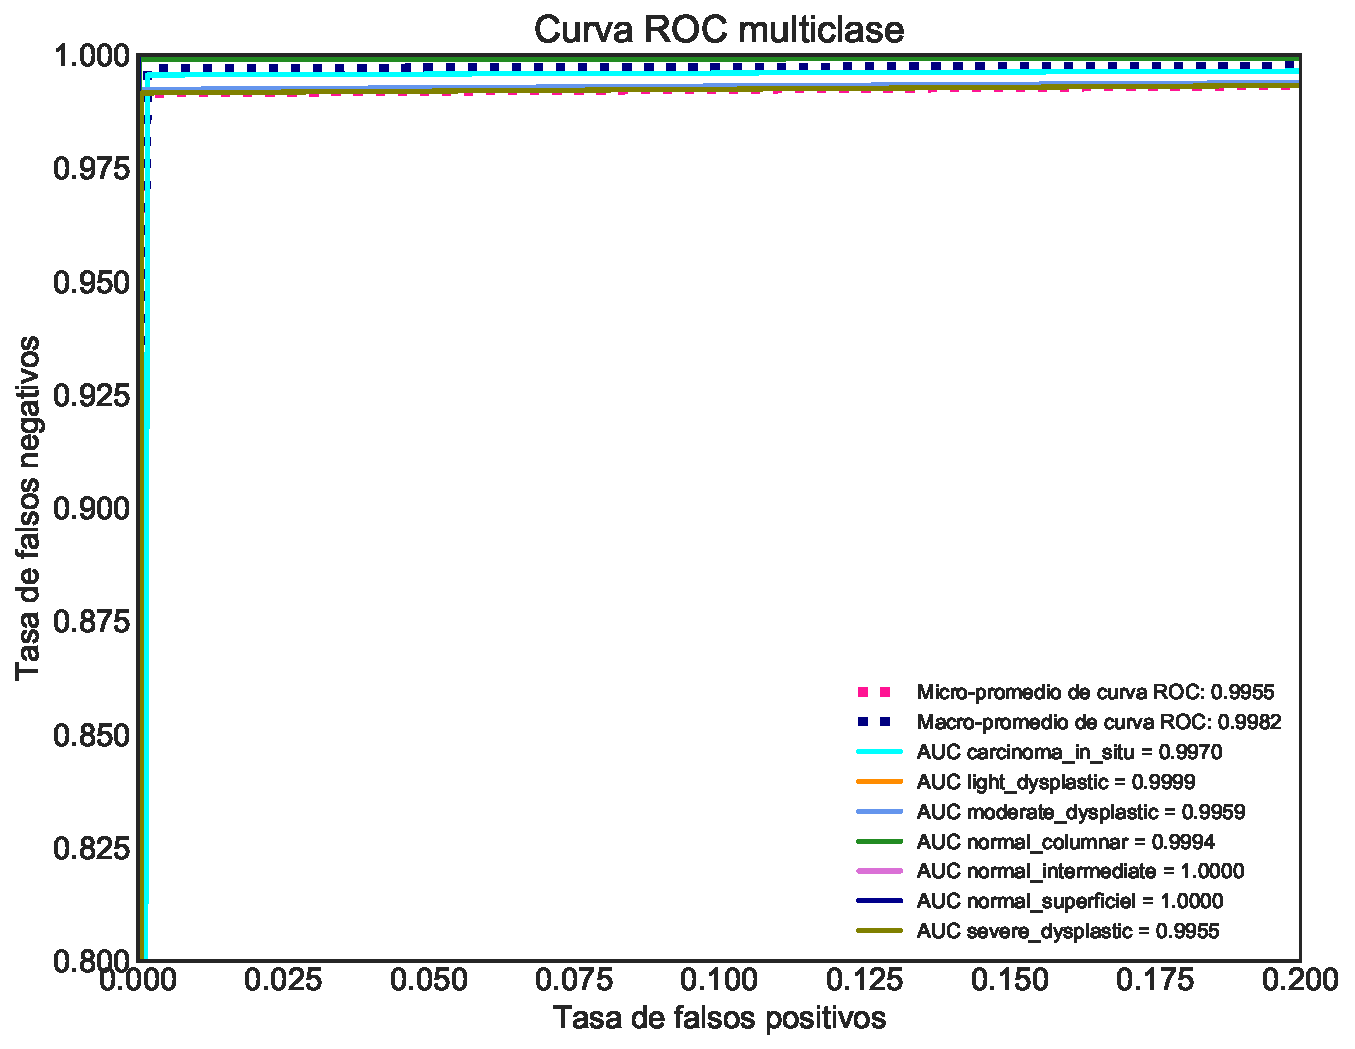
\includegraphics[width=0.8\textwidth]{capitulo_sdac/reporte_7_class/roc_multiclase.pdf}
    \caption{ROC y AUC multi-clase}\label{fig:roc_multi}
\end{figure} 

En la tabla de métricas de diagnóstico (\autoref{tabla:diag_7}), llama la
atención el valor de \emph{None} en las clases \emph{normal\_intermediate} y
\emph{normal\_superficiel}, esto se debe a que tienen cero clasificaciones
erróneas y las fórmulas deben de haber encontrado una división por 0. 

% Please add the following required packages to your document preamble:
% \usepackage{graphicx}
\begin{table}[H]
    \centering
    \resizebox{0.8\textwidth}{!}{%
    \begin{tabular}{llllllll}
    Class & \rot{\shortstack[l]{carcinoma\_in\_situ}} & \rot{\shortstack[l]{light\_dysplastic}} & \rot{\shortstack[l]{moderate\_dysplastic}} & \rot{\shortstack[l]{normal\_columnar}} &\rot{\shortstack[l]{normal\_intermediate}} & \rot{\shortstack[l]{normal\_superficiel}} & \rot{\shortstack[l]{severe\_dysplastic}} \\ \midrule
    PLR & 610.12117 & 4226.5 & 2146.72087 & 3862.56863 & None & None & 1641.25169 \\
    NLR & 0.00447 & 0 & 0.00764 & 0.00102 & 0 & 0 & 0.00843 \\
    DOR & 136444.1429 & None & 280822.2188 & 3797853.75 & None & None & 194644.2 \\
    DP & 2.83105 & None & 3.00388 & 3.62749 & None & None & 2.91611 \\
    IS & 3.09648 & 2.95721 & 3.20618 & 2.30052 & 2.80083 & 2.69014 & 2.76294
    \end{tabular}%
    }
    \caption{Métricas de diagnóstico de 7 clases}\label{tabla:diag_7}
    \end{table}

De todas las imágenes mal clasificadas del problema de siete clases, tomamos
unas muestras de cada una para poder visualizar lo errado de la clasificación e
intentar distinguir para posteriores experimentos. Se muestrearon solo cuatro
clases ya que son las únicas que tienen malas clasificaciones. Podemos ver en la
\autoref{fig:muestreo_7} que las características morfológicas de las células mal
clasificadas son bastantes similares, lo cual hace obvia la razón por la cual
fueron mal clasificadas. Ninguna célula anormal fue clasificada como normal pero
si una célula normal fue clasificada como anormal.

\begin{figure}[H]
    \centering
    \includegraphics[width=0.8\textwidth]{capitulo_sdac/reporte_7_class/muestras_erroneas.pdf}
    \caption{Muestreo de pruebas mal clasificadas para 7 clases}\label{fig:muestreo_7}
\end{figure}

\subsubsection{Segmentación semántica}

Como vimos anteriormente, la diferencia entre las métricas y la pérdida en las fases de validación
y entrenamiento es una medida para saber que tan bueno es el modelo para generalizar. 

La~\autoref{fig:caja_total2_seg} nos muestra el gráfico de caja para las
métricas y la pérdida, respectivamente. Podemos ver que la exactitud casi no
varia, pero la métrica que nos importa IOU tiene como mínimo casi 50\% en
entrenamiento. Ambas pérdidas se comportan de manera muy similar, otra vez,
demostrando el buen entrenamiento del modelo.

\begin{figure}[H]
    \centering
    \begin{subfigure}[b]{0.8\textwidth}
        \centering
       \includegraphics[width=1\textwidth,height=7cm]{capitulo_sdac/boxen.pdf}
       \caption{Gráfico de caja de métricas}\label{fig:caja_acc2_seg} 
    \end{subfigure}

    \begin{subfigure}[b]{0.8\textwidth}
        \centering
       \includegraphics[width=1\textwidth,height=7cm]{capitulo_sdac/boxen_loss.pdf}
       \caption{Gráfico de caja de pérdida}\label{fig:caja_loss2_seg}
    \end{subfigure}
    \caption{Gráficos de caja}\label{fig:caja_total2_seg}
\end{figure}

En la~\autoref{fig:caja_total_seg} observamos que la variabilidad es bastante
baja comparando validación y entrenamiento, podemos inferir que el modelo
generaliza correctamente. Los picos en variación corresponden a los picos
observados en la fase de entrenamiento. La métrica IOU varía más puesto que es
un análisis de todos los pixeles en una imagen.

\begin{figure}[H]
    \centering
    \begin{subfigure}[b]{0.6\textwidth}
        \centering
       \includegraphics[width=1\textwidth]{capitulo_sdac/box_mejorada_iou.pdf}
       \caption{Variación en IOU}\label{fig:caja_acc_seg} 
    \end{subfigure}

    \begin{subfigure}[b]{0.6\textwidth}
        \centering
       \includegraphics[width=1\textwidth]{capitulo_sdac/box_mejorada_loss.pdf}
       \caption{Variación en la pérdida}\label{fig:caja_loss_seg}
    \end{subfigure}
    \caption{Gráfica de caja de la variación en segmentación}\label{fig:caja_total_seg}
\end{figure}

El modelo se comporta mejor conforme pasan las épocas y es posible mejorar el
rendimiento del mismo incrementando los hiper-parámetros que controlan el
entrenamiento. No fue posible incrementar a 64 el tamaño del lote debido a
problemas con la memoria derivados de la naturaleza de la arquitectura. Es
probable que se requiera reentrenar el modelo para poder lidiar con imágenes con
mucho más ruido que las utilizadas, esto depende de la correcta anotación de la
base de datos de laminilla, lo cual se pretende hacer mediante algoritmos
tradicionales de Procesamiento Digital de Imágenes en un futuro.

Después de la validación hemos tomado \(n = 10\) muestras para mostrar
gráficamente la clasificación de los pixeles y estimar visualmente el
rendimiento del experimento. La~\autoref{fig:mascaras} nos muestra claramente
que el algoritmo es capaz de distinguir correctamente entre el núcleo, el
citoplasma y el fondo de la imagen. Se puede observar que el mayor problema del
algoritmo es la tasa de falsos positivos, mientras que los falsos negativos son
relativamente escasos. Se puede asegurar que el algoritmo clasifica pixeles
entre núcleo y resto de manera muy eficaz.

\begin{figure}[H]
    \centering
    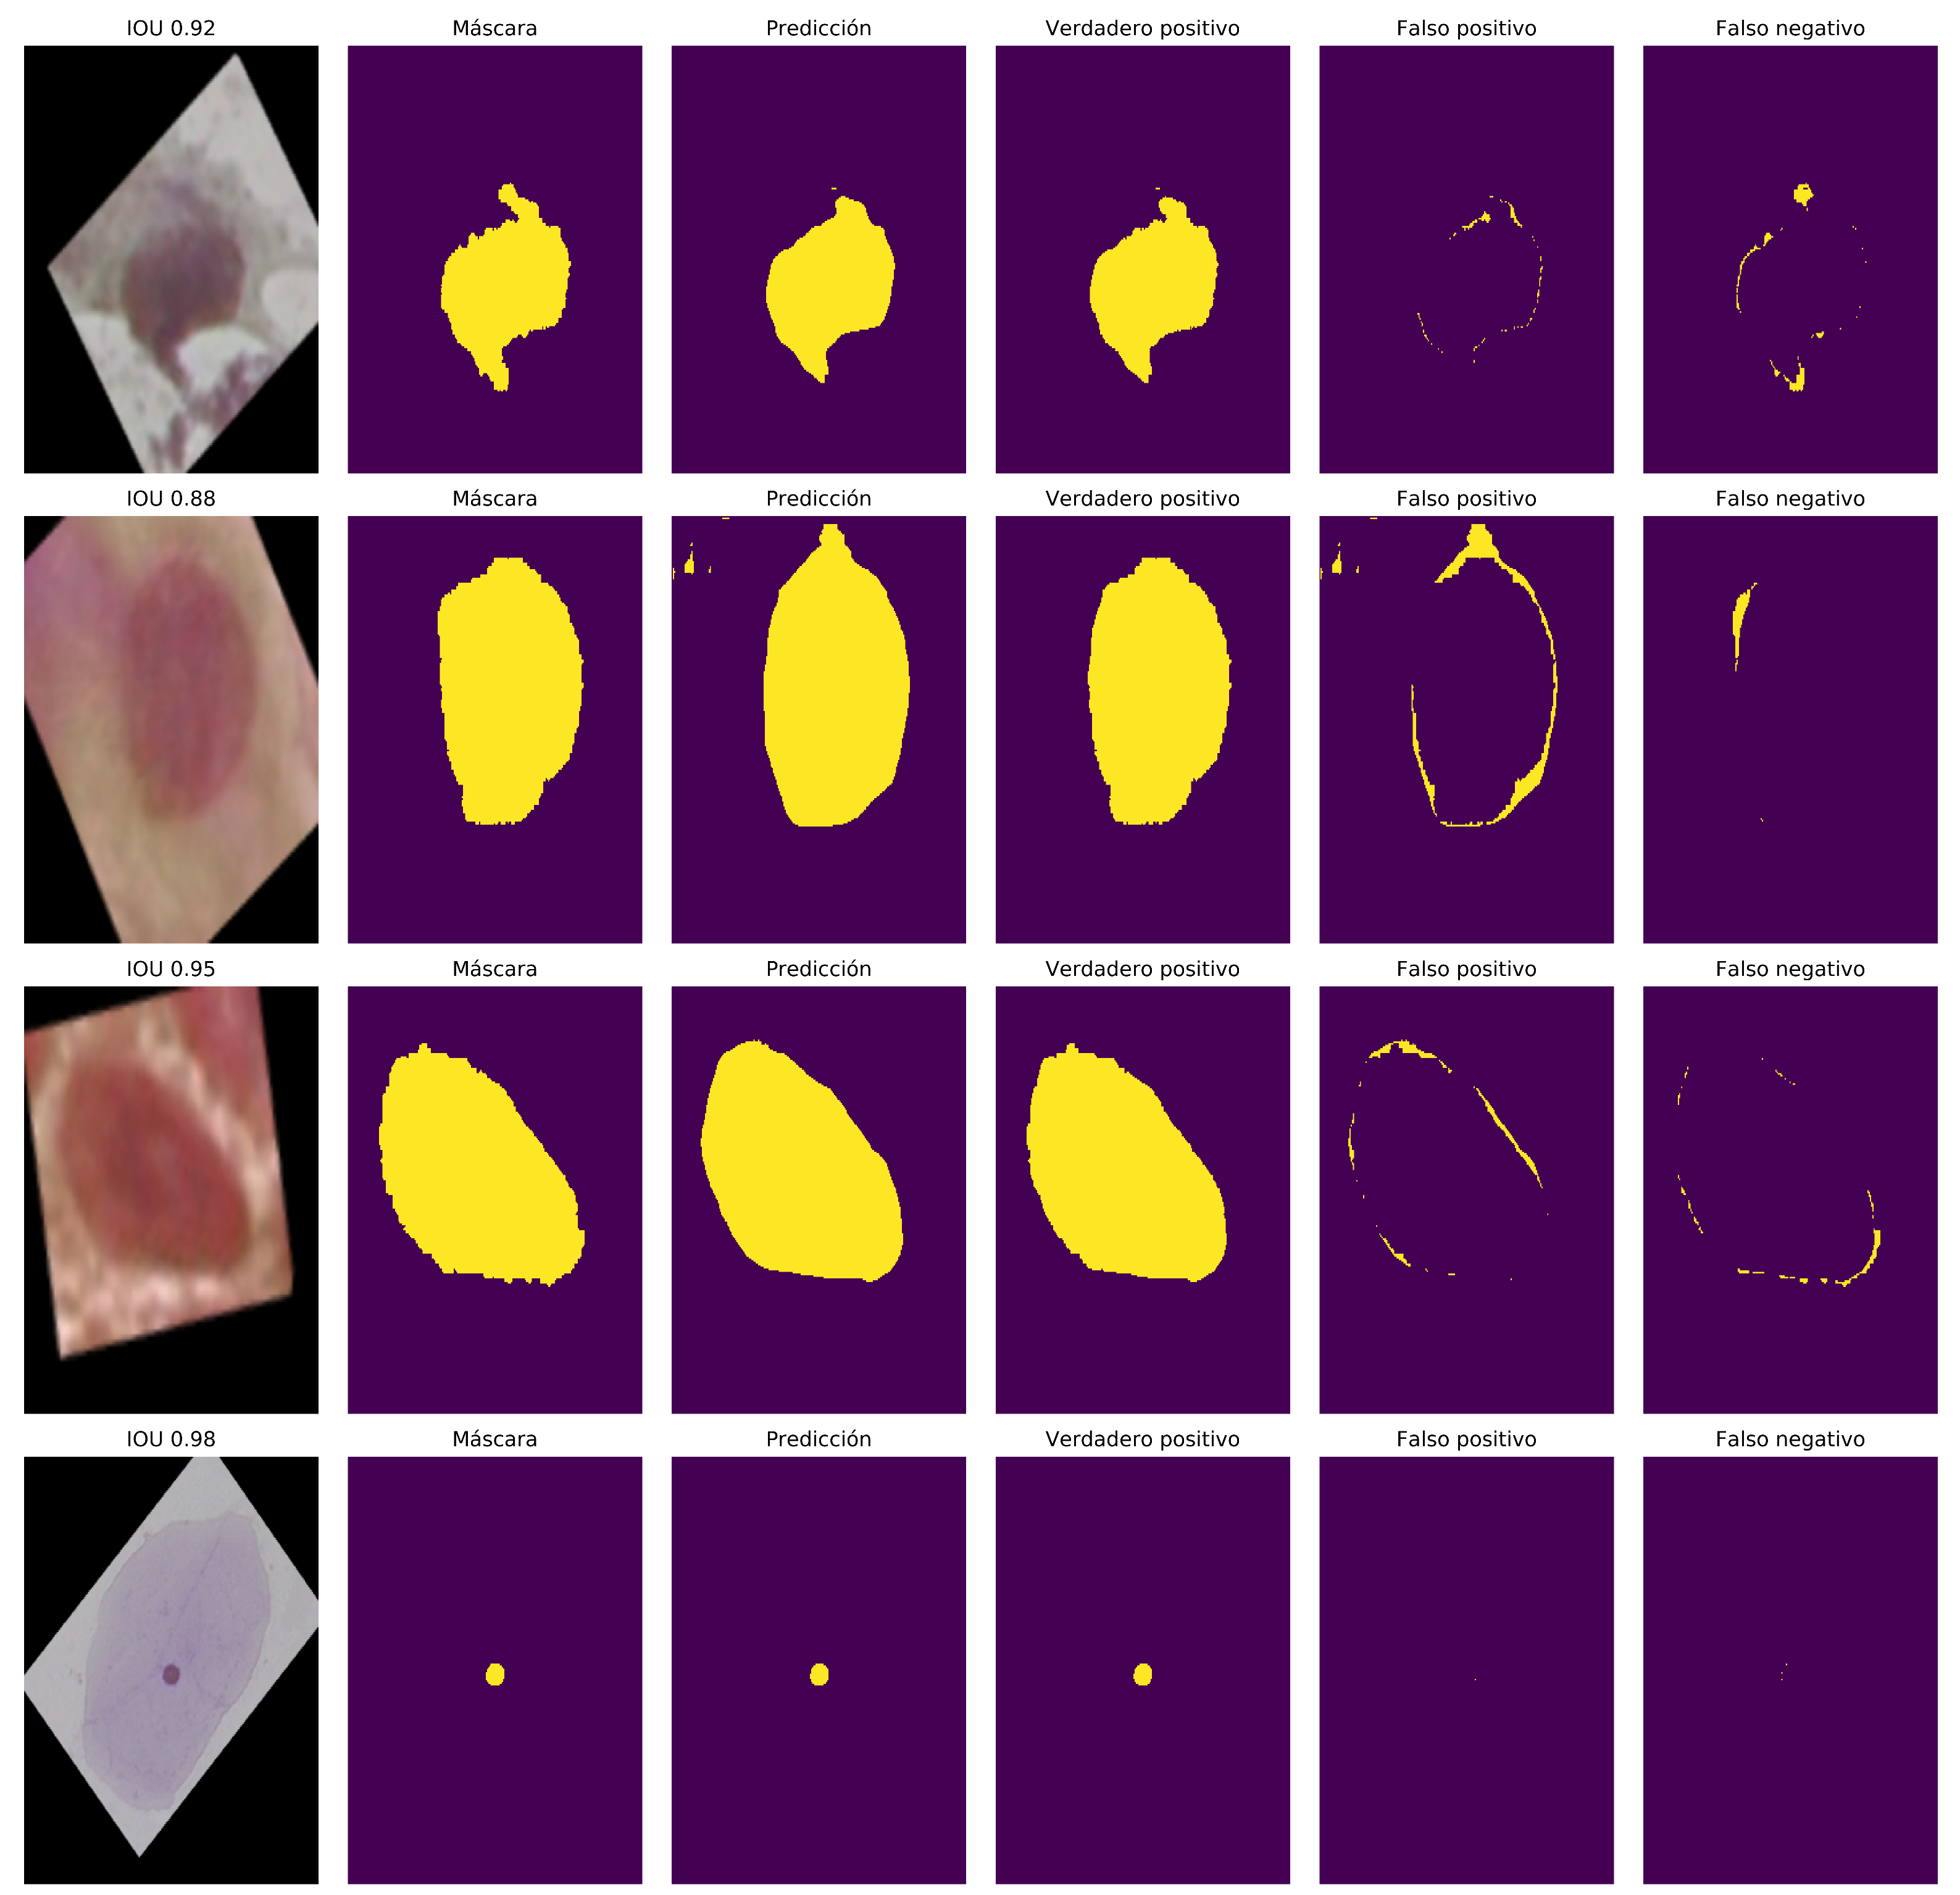
\includegraphics[width=0.8\textwidth]{capitulo_sdac/muestreo_mascaras_segmentacion}
    \caption{Muestreo de máscaras de validación}\label{fig:mascaras}
\end{figure}

Estas pruebas fueron realizadas en un conjunto de datos externo que contiene
imágenes que campo amplio de una laminilla de Papanicolau. Para poder observar
el rendimiento de la segmentación en una aplicación similar a la real
(\autoref{fig:laminilla}). Si bien el rendimiento no es perfecto, debido a la
revisión que hace la red por cada pixel de la imagen, se nota que detecta
relativamente bien el núcleo dentro de la imagen; tomando en cuenta que estas
imágenes si tienen múltiples células y que la red fue entrenada con imágenes que
contienen solo una.

\begin{figure}[H]
    \centering
    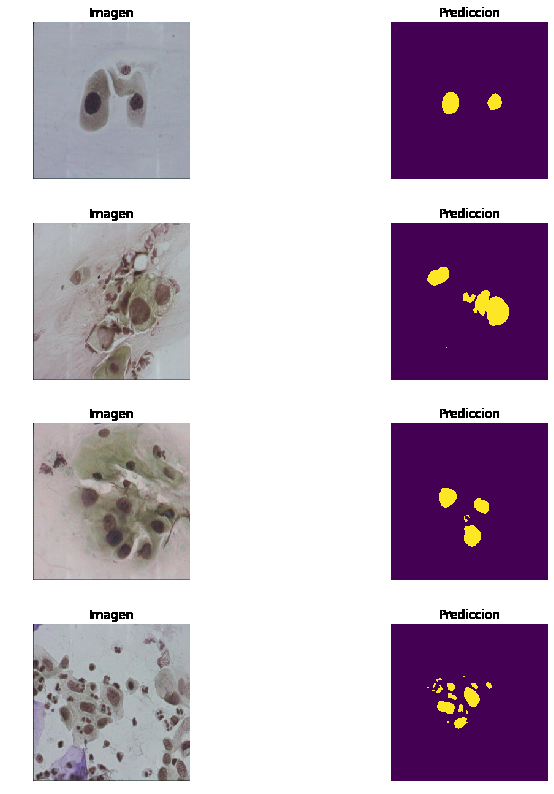
\includegraphics[width=0.5\textwidth]{capitulo_sdac/test_segmentacion}
    \caption{Pruebas en imagen de laminilla}\label{fig:laminilla}
\end{figure}

\subsection{Análisis del modelo y comprobación de supuestos}

Esta etapa no está estipulada dentro de la metodología básica para
\hyperlink{abbr}{ML}, sin embargo, los modelos de \hyperlink{abbr}{DL} como las
\hyperlink{abbr}{ConvNets} carecen de interpretabilidad. Esta capacidad está
presente en algoritmos como los árboles de decisión donde rastrear la serie de
decisiones que tomó el algoritmo para la clasificación final es tan fácil como
seguir las ramas de vuelta.

Tenemos que analizar como el \hyperlink{abbr}{TL} actúa en las capas de la arquitectura para
detectar patrones y conectar esto a lo que ven las capas subsecuentes y finales
que son las que se entrenaron. Vislumbrar que ve cada filtro de cada capa nos
permitirá saber que patrones está captando la red para hacer su clasificación y
por consiguiente el diagnóstico.

Los supuestos para llevar a cabo los experimentos de clasificación de imágenes
fueron los siguientes:

\begin{itemize}
  \item El núcleo celular contiene suficiente información para diferenciar entre
  los tipos de célula citológica cervical.
  \item Las técnicas de aumento de datos no inciden en la decisión del
  algoritmo.
  \item La red neuronal es capaz de diferenciar correctamente en un espacio
  multidimensional entre los tipos de célula.
\end{itemize}

El primer supuesto guio el desarrollo de los algoritmos de aumentación de datos
y la premisa que sustenta la investigación. 

El segundo tiene que ver específicamente con las características de la imagen
aumentada; se requiere saber si los pixeles extras añadidos a la imagen en el
proceso de rotación afecta la inferencia del algoritmo.

El tercero relaciona el espacio multidimensional generado por el algoritmo con
la relación bidimensional de cada ejemplo en comparación a los demás.

Para probar los supuestos, se utilizaron técnicas novedosas de análisis,
optimizaciones específicas de gradiente para cada capa, métodos de visualización
híbridos de visión por computadora y algoritmos de reducción de la
dimensionalidad.

\subsubsection{Análisis de las capas del modelo}

La justificación por la cual no se realizaron experimentos para encontrar una
arquitectura particular para el problema es el \hyperlink{abbr}{TL}. Esta forma de
construir nuevos modelos de manera incremental basándose en conocimiento
anterior es el motor que guía no solo el aprendizaje humano sino toda la
ciencia.

Para entender como ayuda el \hyperlink{abbr}{TL}, en particular la arquitectura
VGG19 entrenada en \emph{ImageNet} al problema expuesto en esta tesis. Mostramos
una selección aleatoria, de cierto número de capas, de los filtros que se
aplican a la imagen al transitar por las capas de la red. 

La~\autoref{fig:filtros} muestra los filtros de algunas capas de la primera a
las capas superiores. Los filtros de las capas inferiores tienden a buscar
patrones sencillos como colores y su relación con la región de la imagen.
Subsecuentemente, vemos que la capas \emph{block2\_conv2} y \emph{block3\_conv1}
detectan patrones más complejos y granulados que detectan patrones como líneas
verticales o bordes. Es en la capa \emph{block4\_conv4} que podemos ver patrones
sumamente complejos y difíciles de interpretar.

\begin{figure}[H] 
  \begin{subfigure}[b]{0.5\linewidth}
    \centering
    \includegraphics[width=0.75\linewidth]{capitulo_sdac/filtros-block1_conv1.pdf} 
    \caption{Filtros block1\_conv1}\label{fig7:aa}
    \vspace{4ex}
  \end{subfigure}%% 
  \begin{subfigure}[b]{0.5\linewidth}
    \centering
    \includegraphics[width=0.75\linewidth]{capitulo_sdac/filtros-block2_conv2.pdf} 
    \caption{Filtros block2\_conv2}\label{fig7:bb}
    \vspace{4ex}
  \end{subfigure} 
  \begin{subfigure}[b]{0.5\linewidth}
    \centering
    \includegraphics[width=0.75\linewidth]{capitulo_sdac/filtros-block3_conv1.pdf} 
    \caption{Filtros block3\_conv1}\label{fig7:cc}
  \end{subfigure}%%
  \begin{subfigure}[b]{0.5\linewidth}
    \centering
    \includegraphics[width=0.75\linewidth]{capitulo_sdac/filtros-block4_conv4.pdf} 
    \caption{Filtros block4\_conv4}\label{fig7:dd}
  \end{subfigure} 
  \caption{Visualización de filtros convolucionales}\label{fig:filtros} 
\end{figure}

Finalmente, se muestran (\autoref{fig:convultima}) los filtros de la última capa
\emph{block5\_conv4}, tales filtros muestran una complejidad bastante alta, con
tintes psicodélicos, que muestran las abstracciones que hace la red para poder
interpretar el contenido de una imagen.

\begin{figure}[H] 
  \centering
  \includegraphics[width=0.8\textwidth]{capitulo_sdac/filtros-block5_conv4.pdf}
  \caption{Filtros de la última capa: block5\_conv4}\label{fig:convultima}
\end{figure}

En la~\autoref{fig:inter} se pueden ver las activaciones de todas las capas de
\emph{Max Pooling} de todos los bloques convolucionales que componen nuestra
arquitectura. Se probaron estas activaciones con una célula cancerígena
aleatoria. Se repite el patrón que hemos visto desde las secciones anteriores,
cada capa captura elementos cada vez más abstractos de la imagen. La capa
\emph{Block1\_pool} evidencia la potencia del algoritmo, pudiendo segmentar
correctamente las partes como el núcleo. Los filtros de la capa
\emph{Block5\_pool} se activan en su mayoría, se concluye que el modelo no es ni
tan sencillo ni tan complejo, en dado caso que hubiesen muchos filtros sin
activar, el modelo sería demasiado complejo para la tarea. Quizás sea esta la
razón por la cual otras arquitecturas más grandes no funcionaron para este
problema.

  \begin{figure}[H] % "[t!]" placement specifier just for this example
    \begin{subfigure}{0.40\textwidth}
      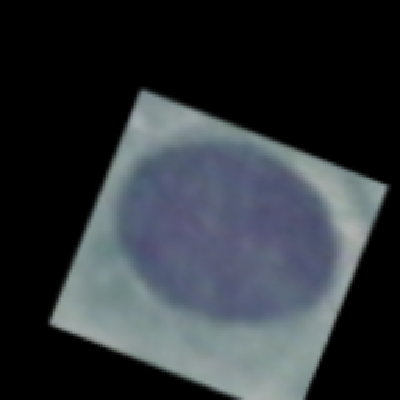
\includegraphics[width=\linewidth]{capitulo_sdac/xcancerseed_activaciones(0).pdf}
      \caption{Block1\_pool}\label{fig:ay}
    \end{subfigure}\hspace*{\fill}
    \begin{subfigure}{0.40\textwidth}
      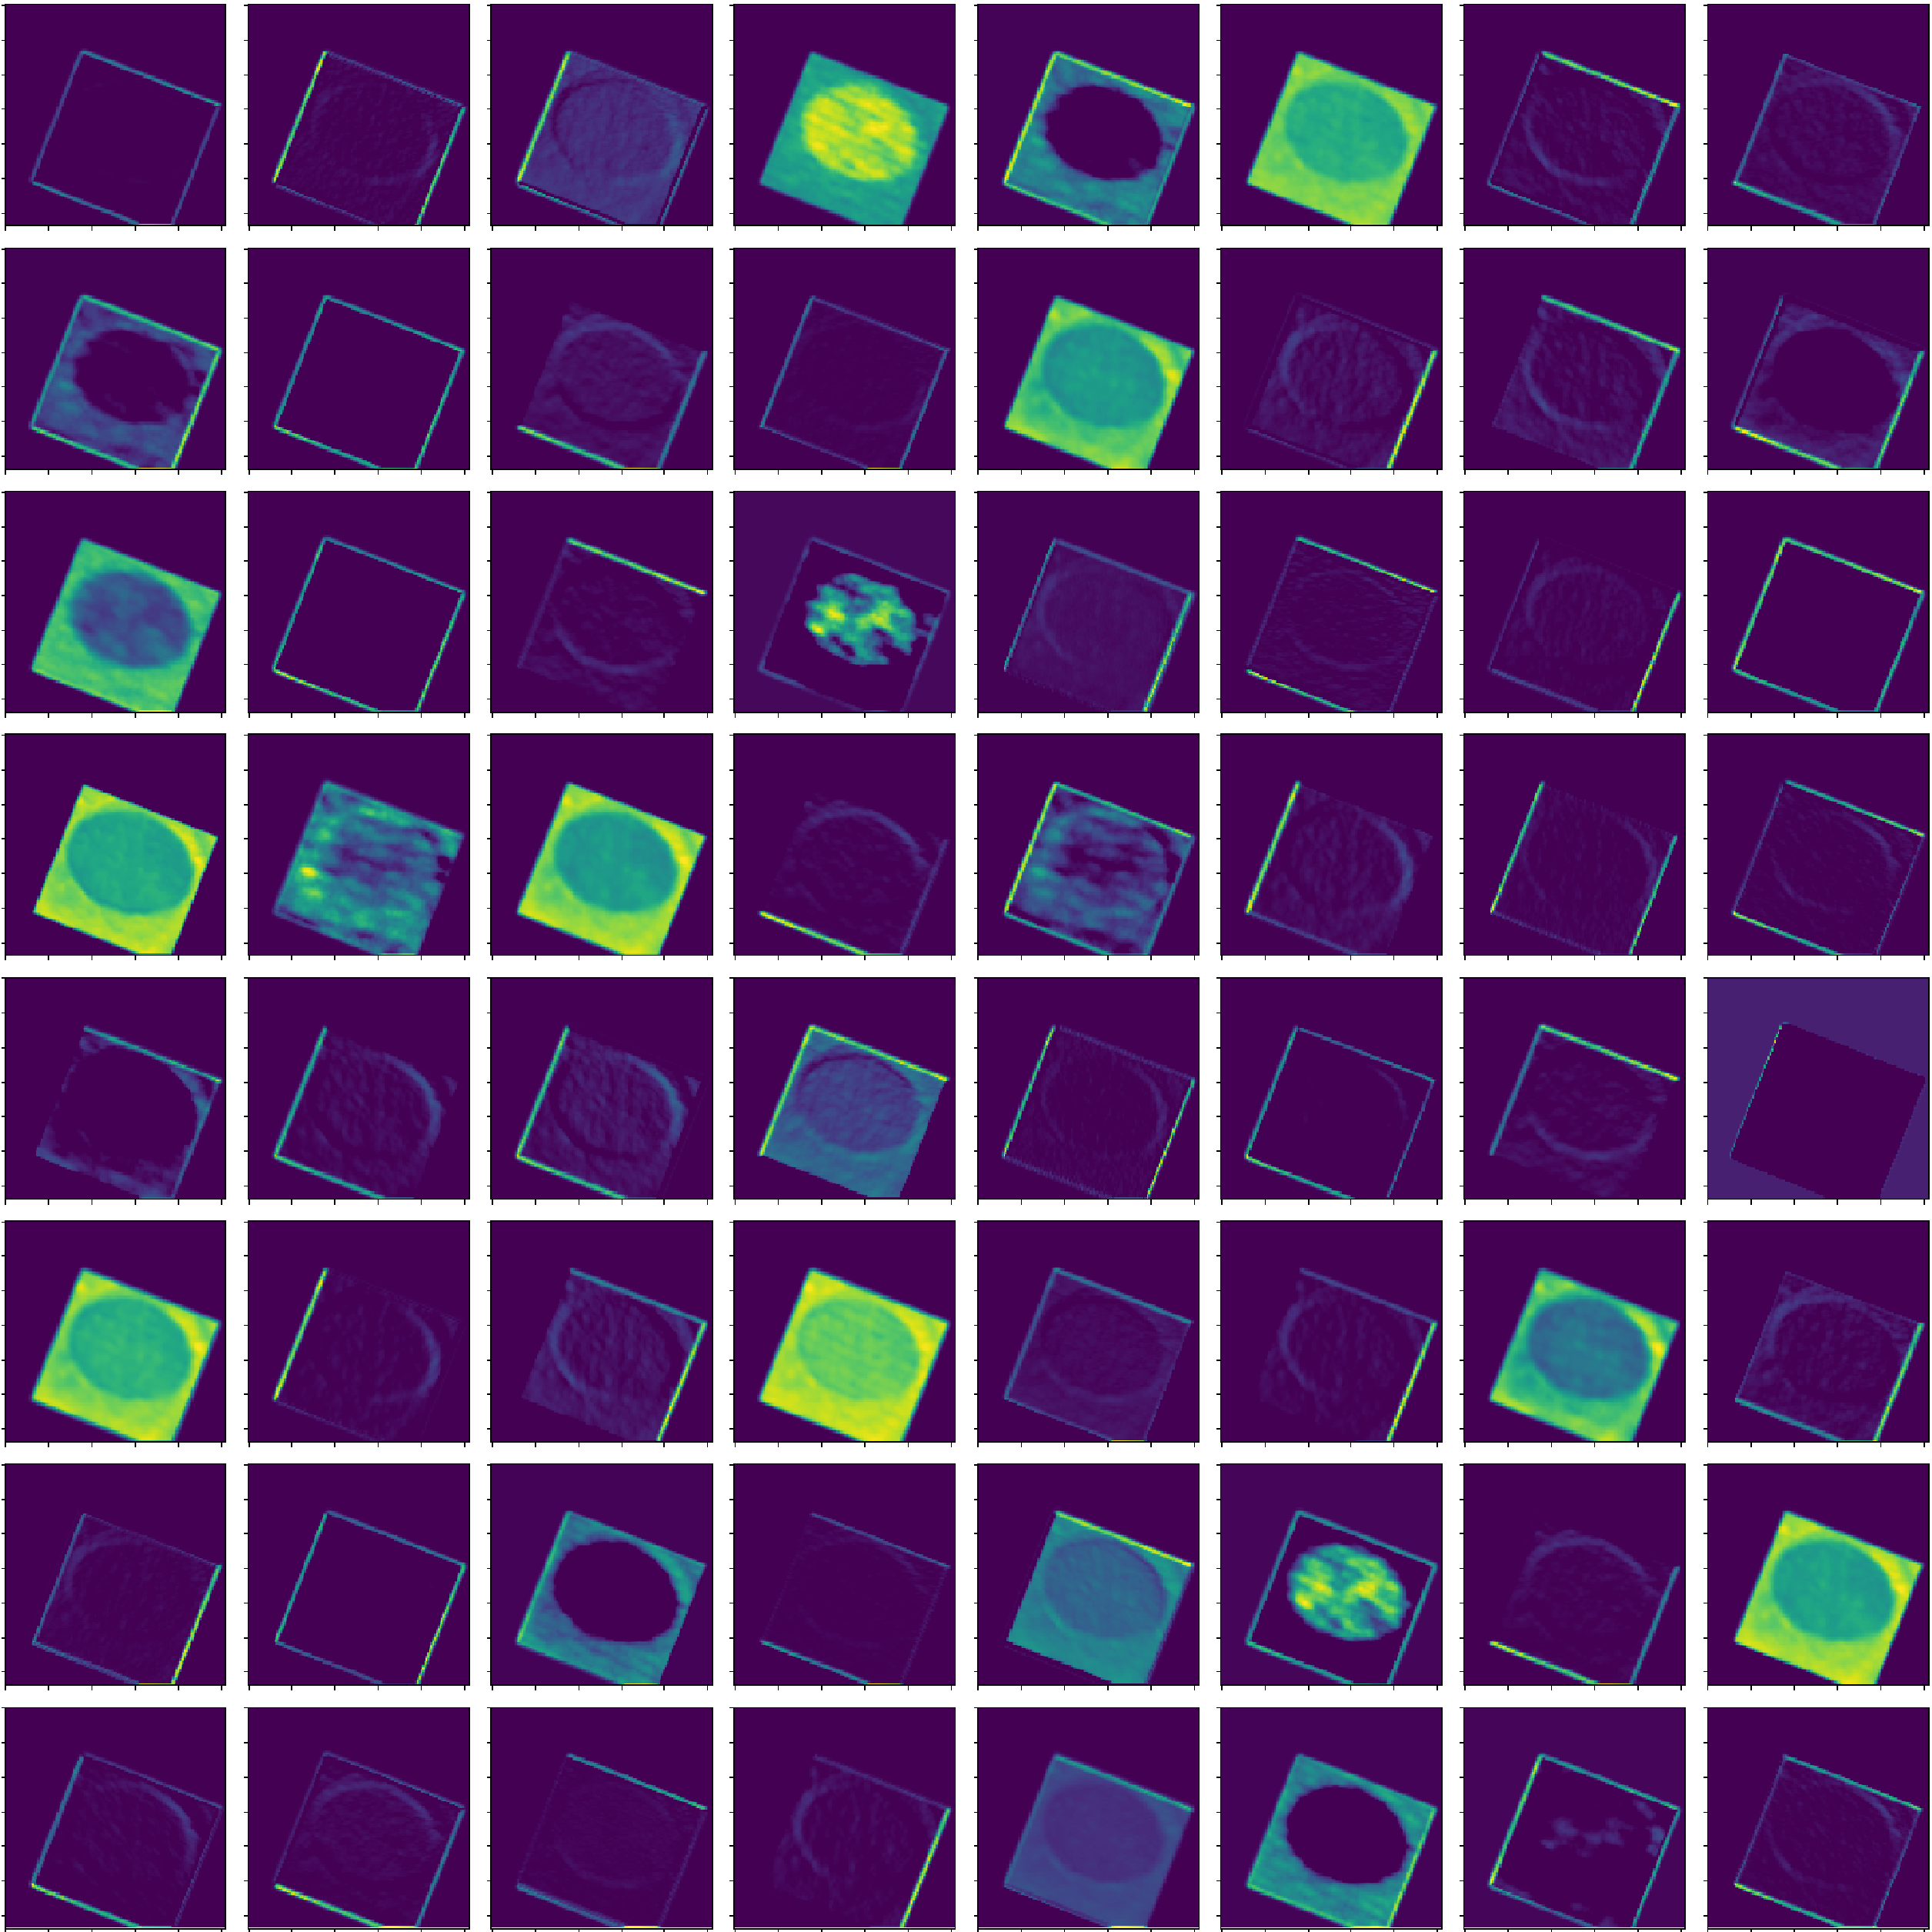
\includegraphics[width=\linewidth]{capitulo_sdac/xcancerblock1_pool-MaxPool_0.pdf}
      \caption{Block1\_pool}\label{fig:by}
    \end{subfigure}
    
    \medskip
    \begin{subfigure}{0.40\textwidth}
      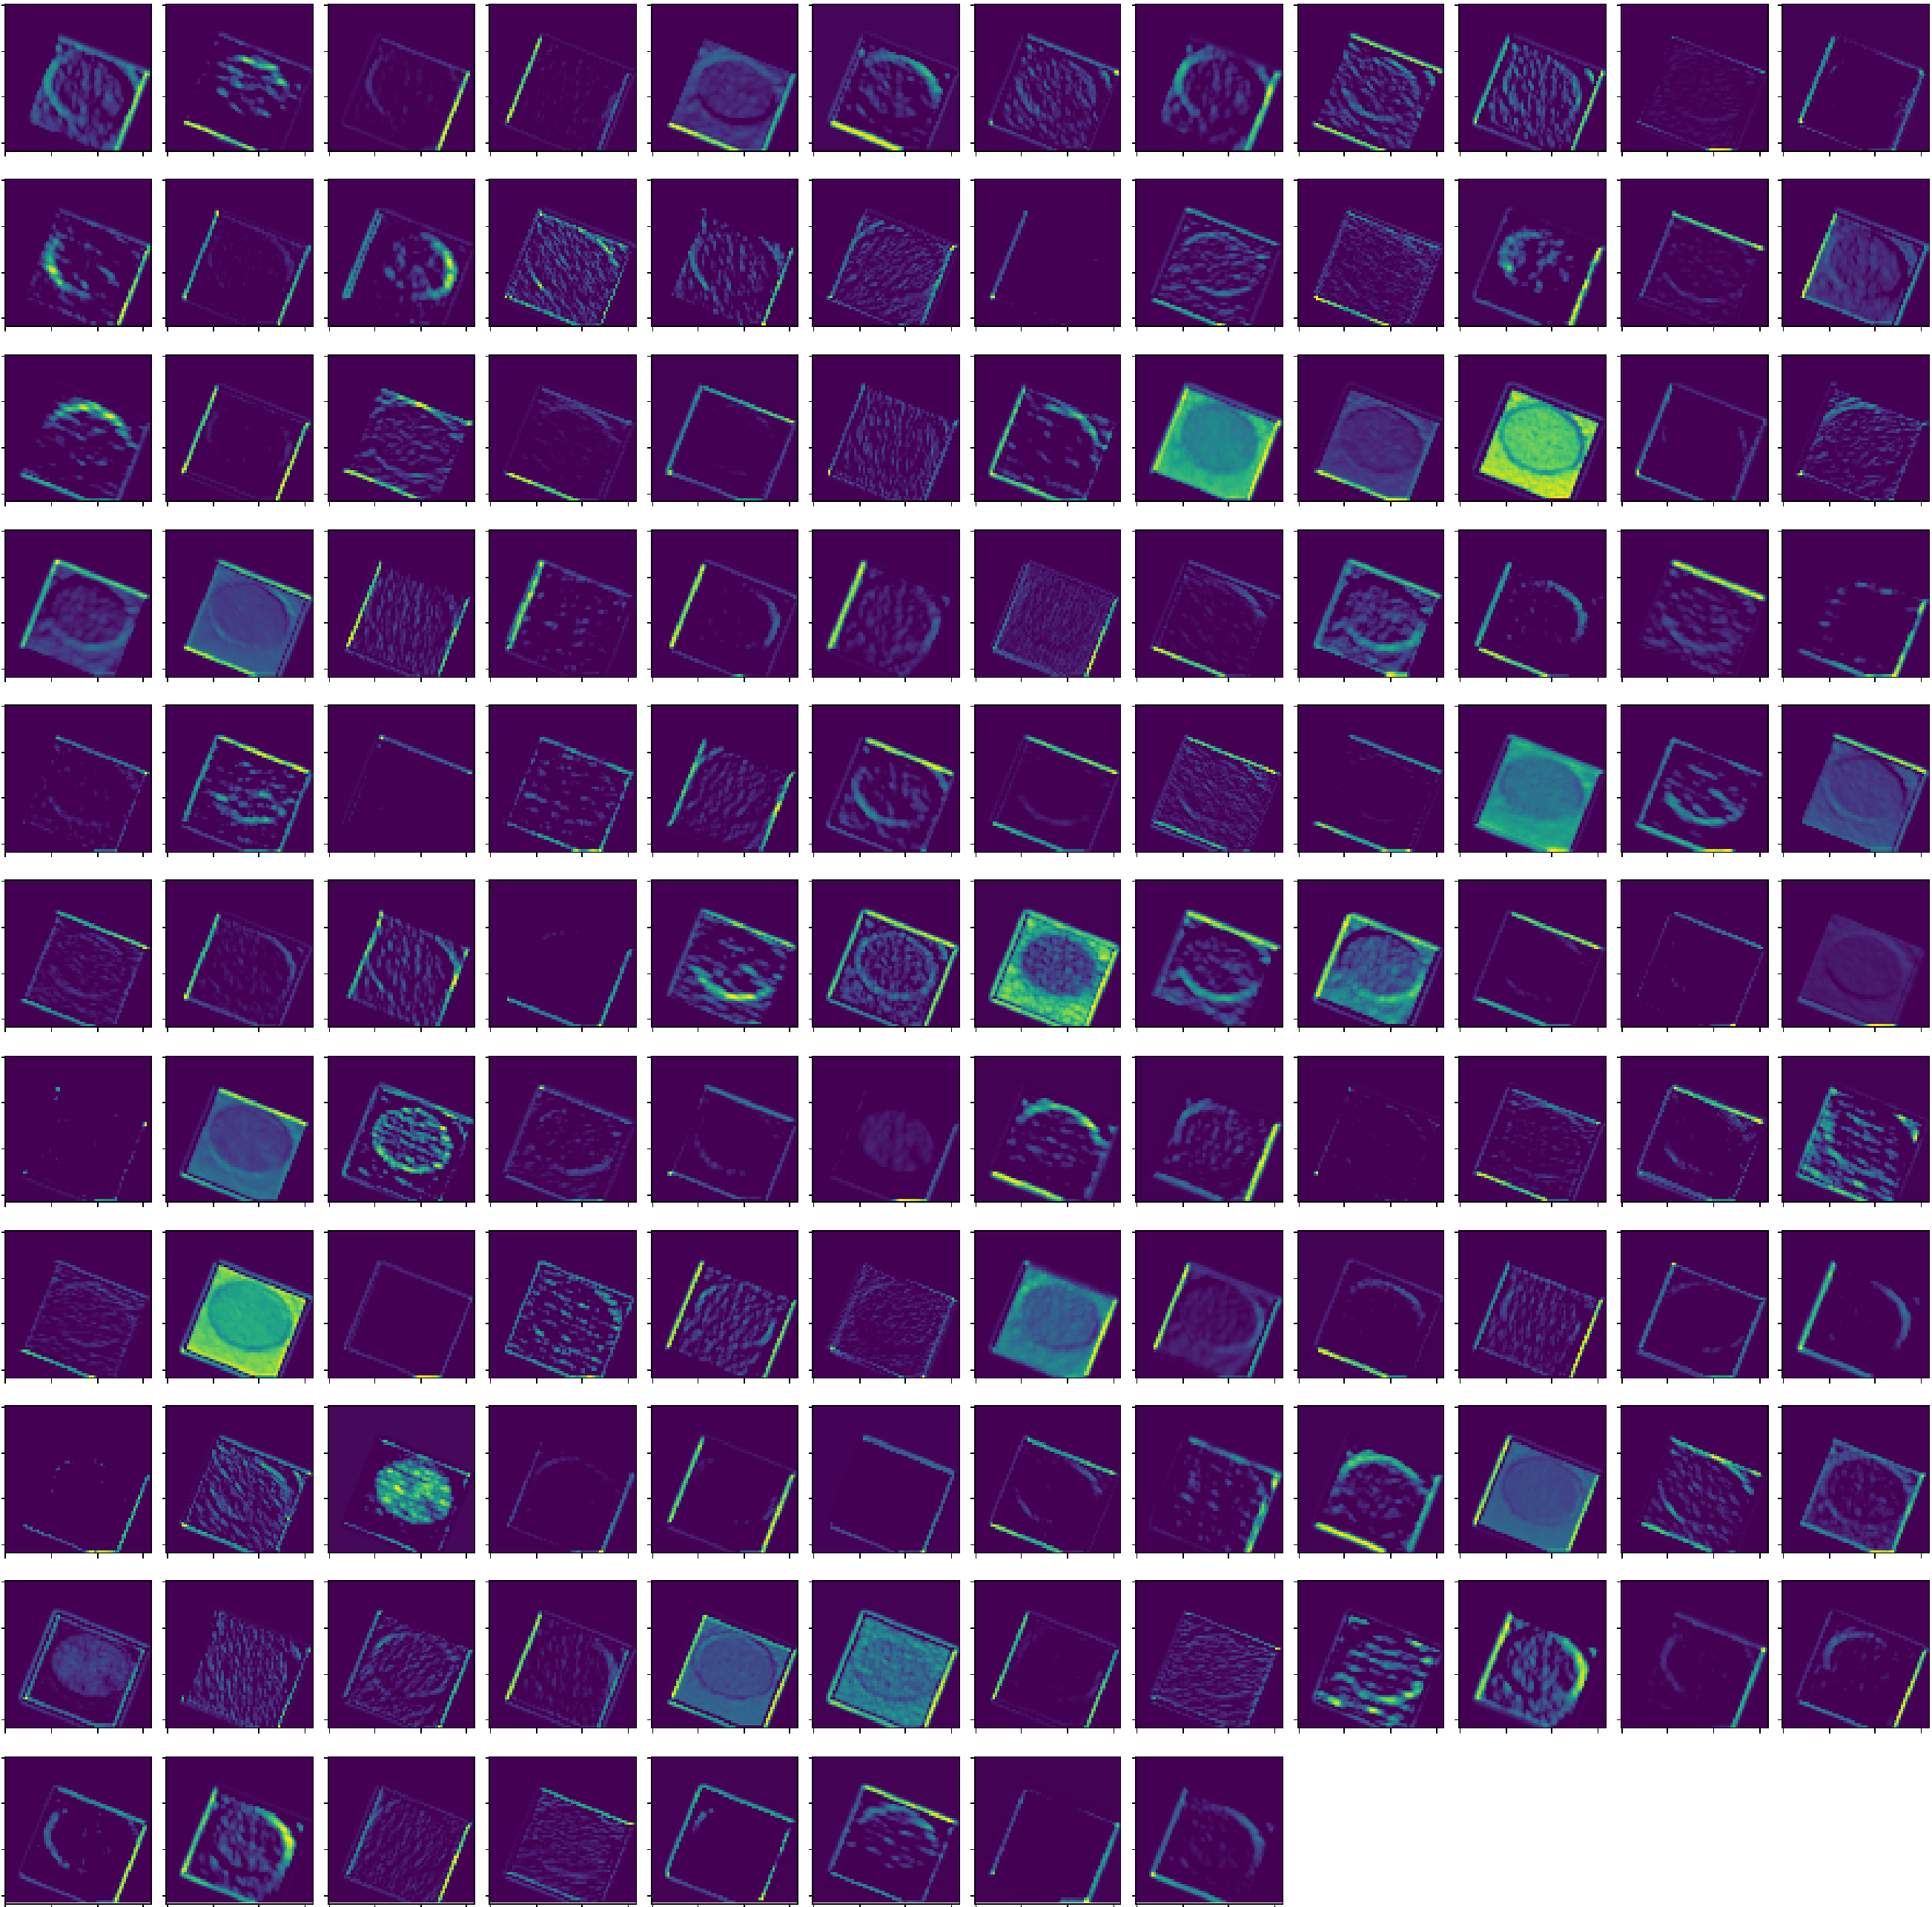
\includegraphics[width=\linewidth]{capitulo_sdac/xcancerblock2_pool-MaxPool_0.pdf}
      \caption{Block2\_pool}\label{fig:cy}
    \end{subfigure}\hspace*{\fill}
    \begin{subfigure}{0.40\textwidth}
      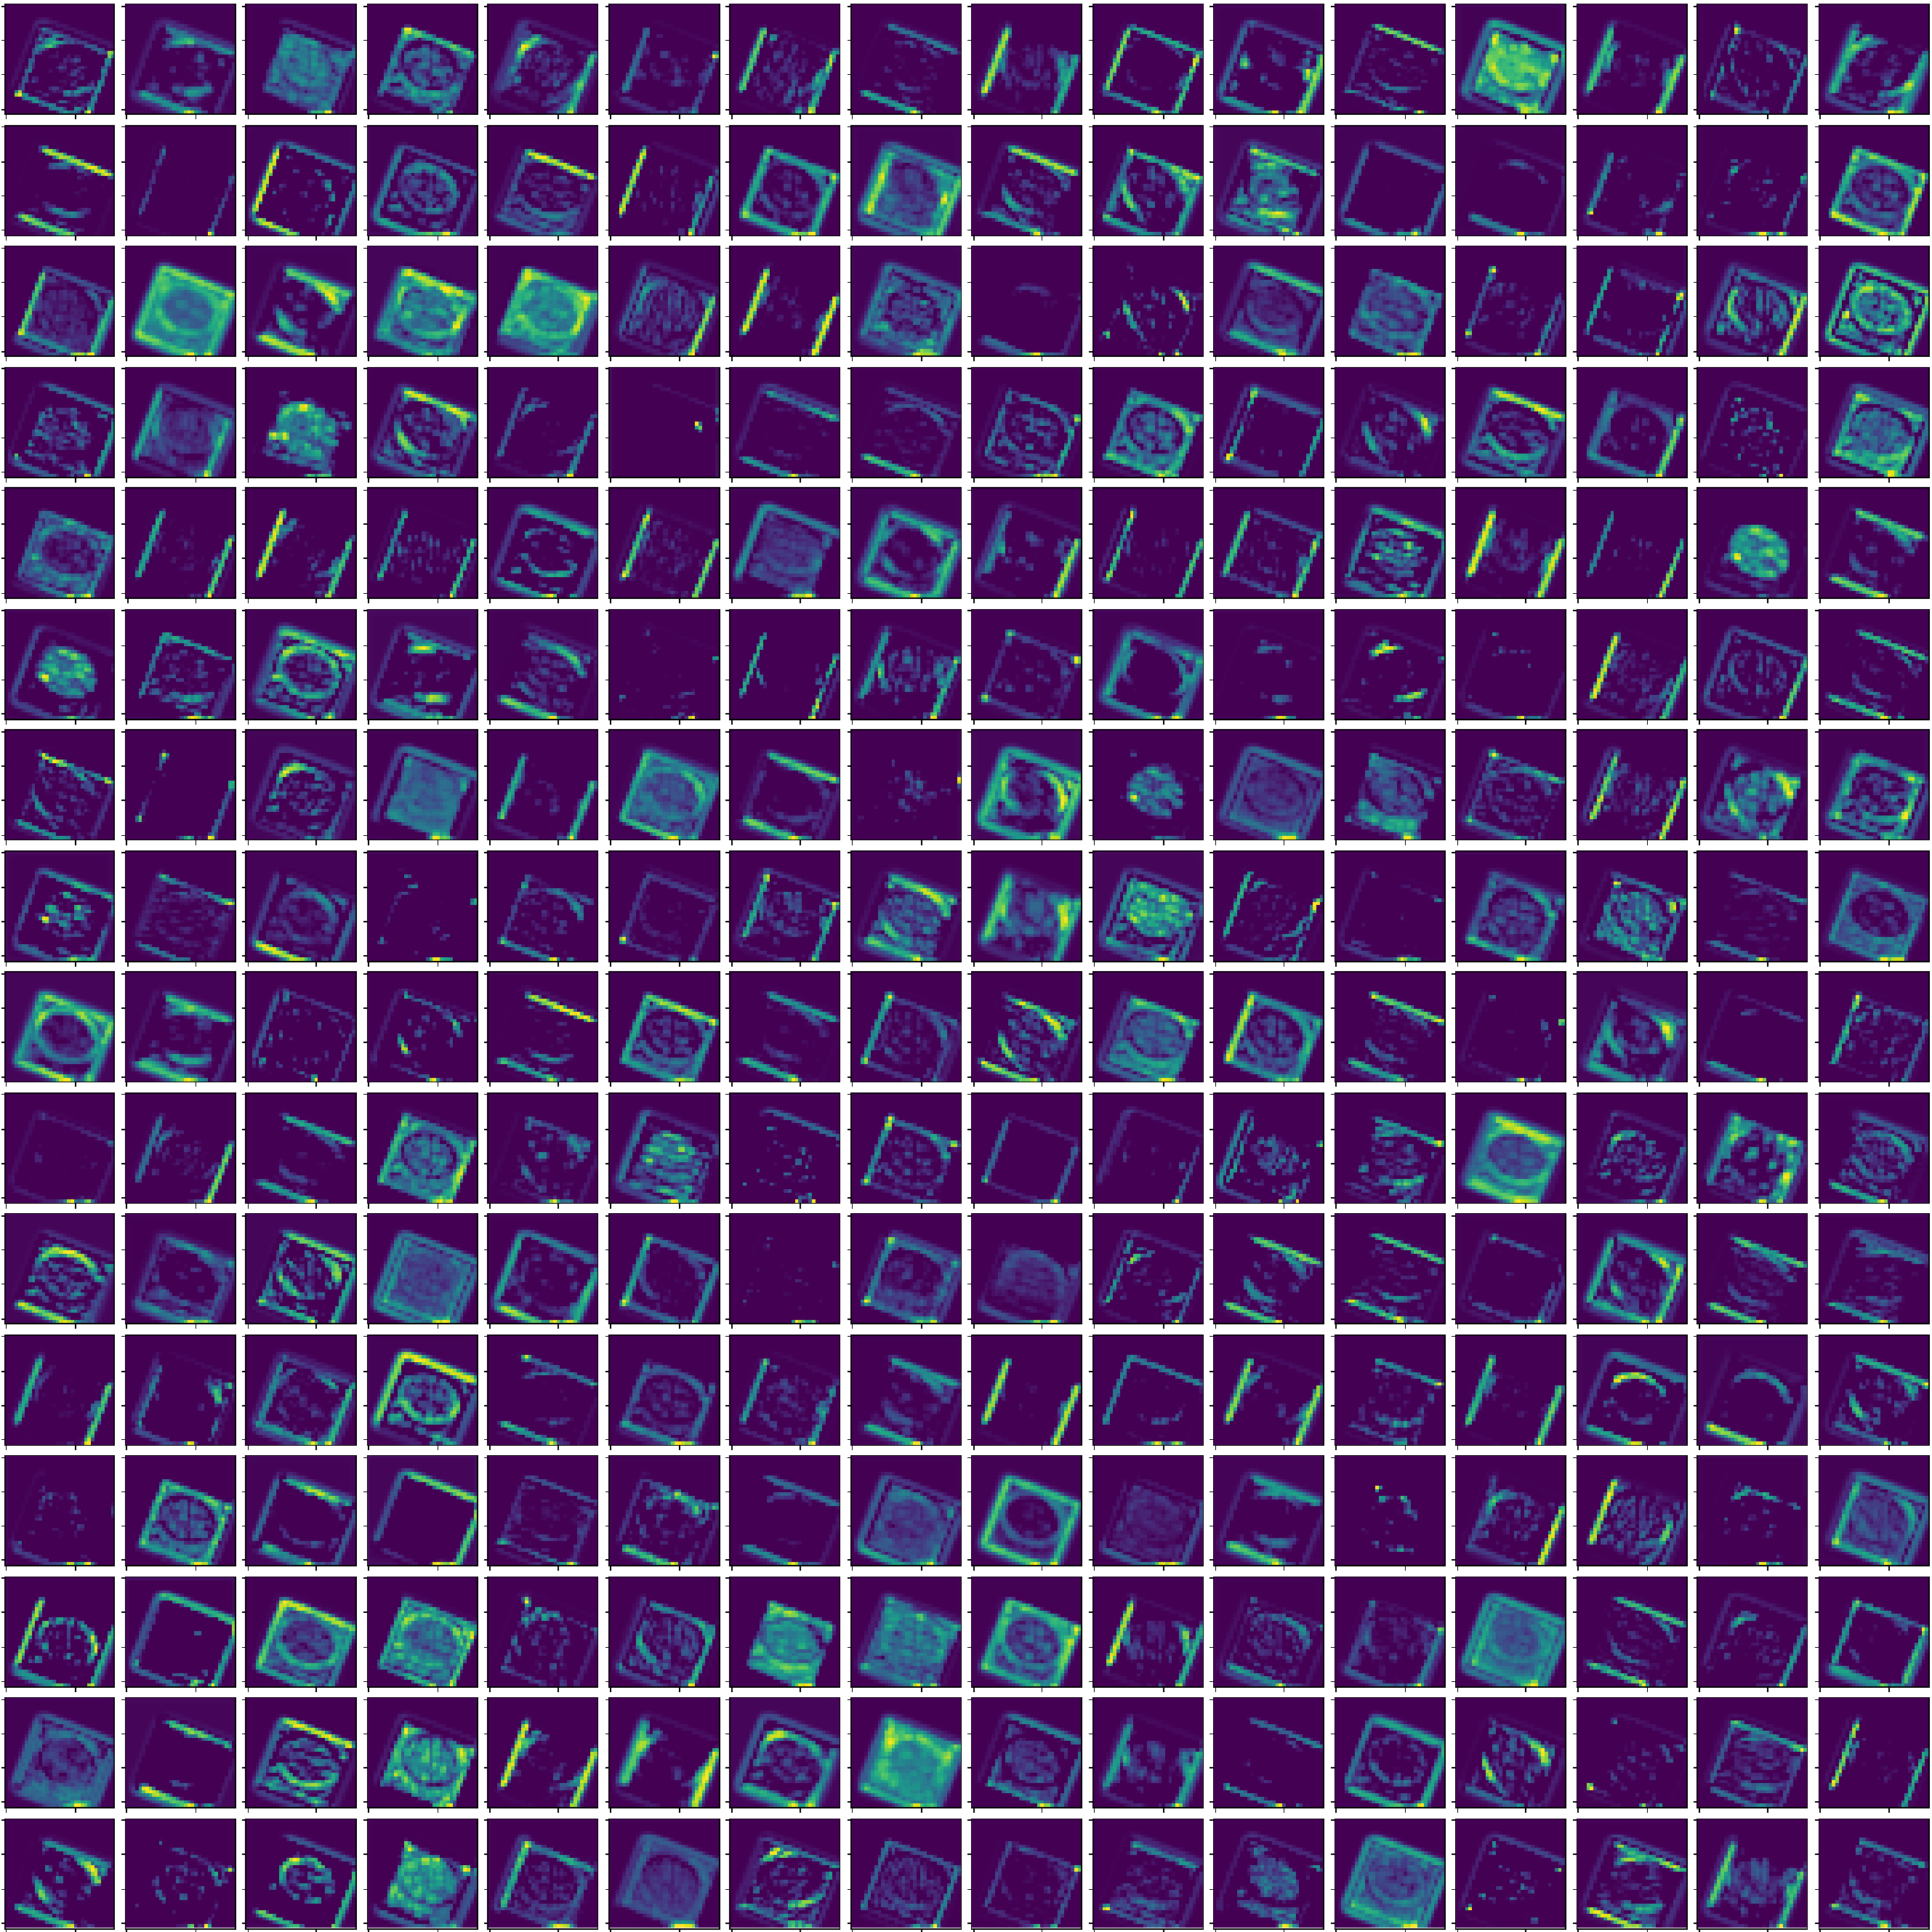
\includegraphics[width=\linewidth]{capitulo_sdac/xcancerblock3_pool-MaxPool_0.pdf}
      \caption{Block3\_pool}\label{fig:dy}
    \end{subfigure}
    
    \medskip
    \begin{subfigure}{0.40\textwidth}
      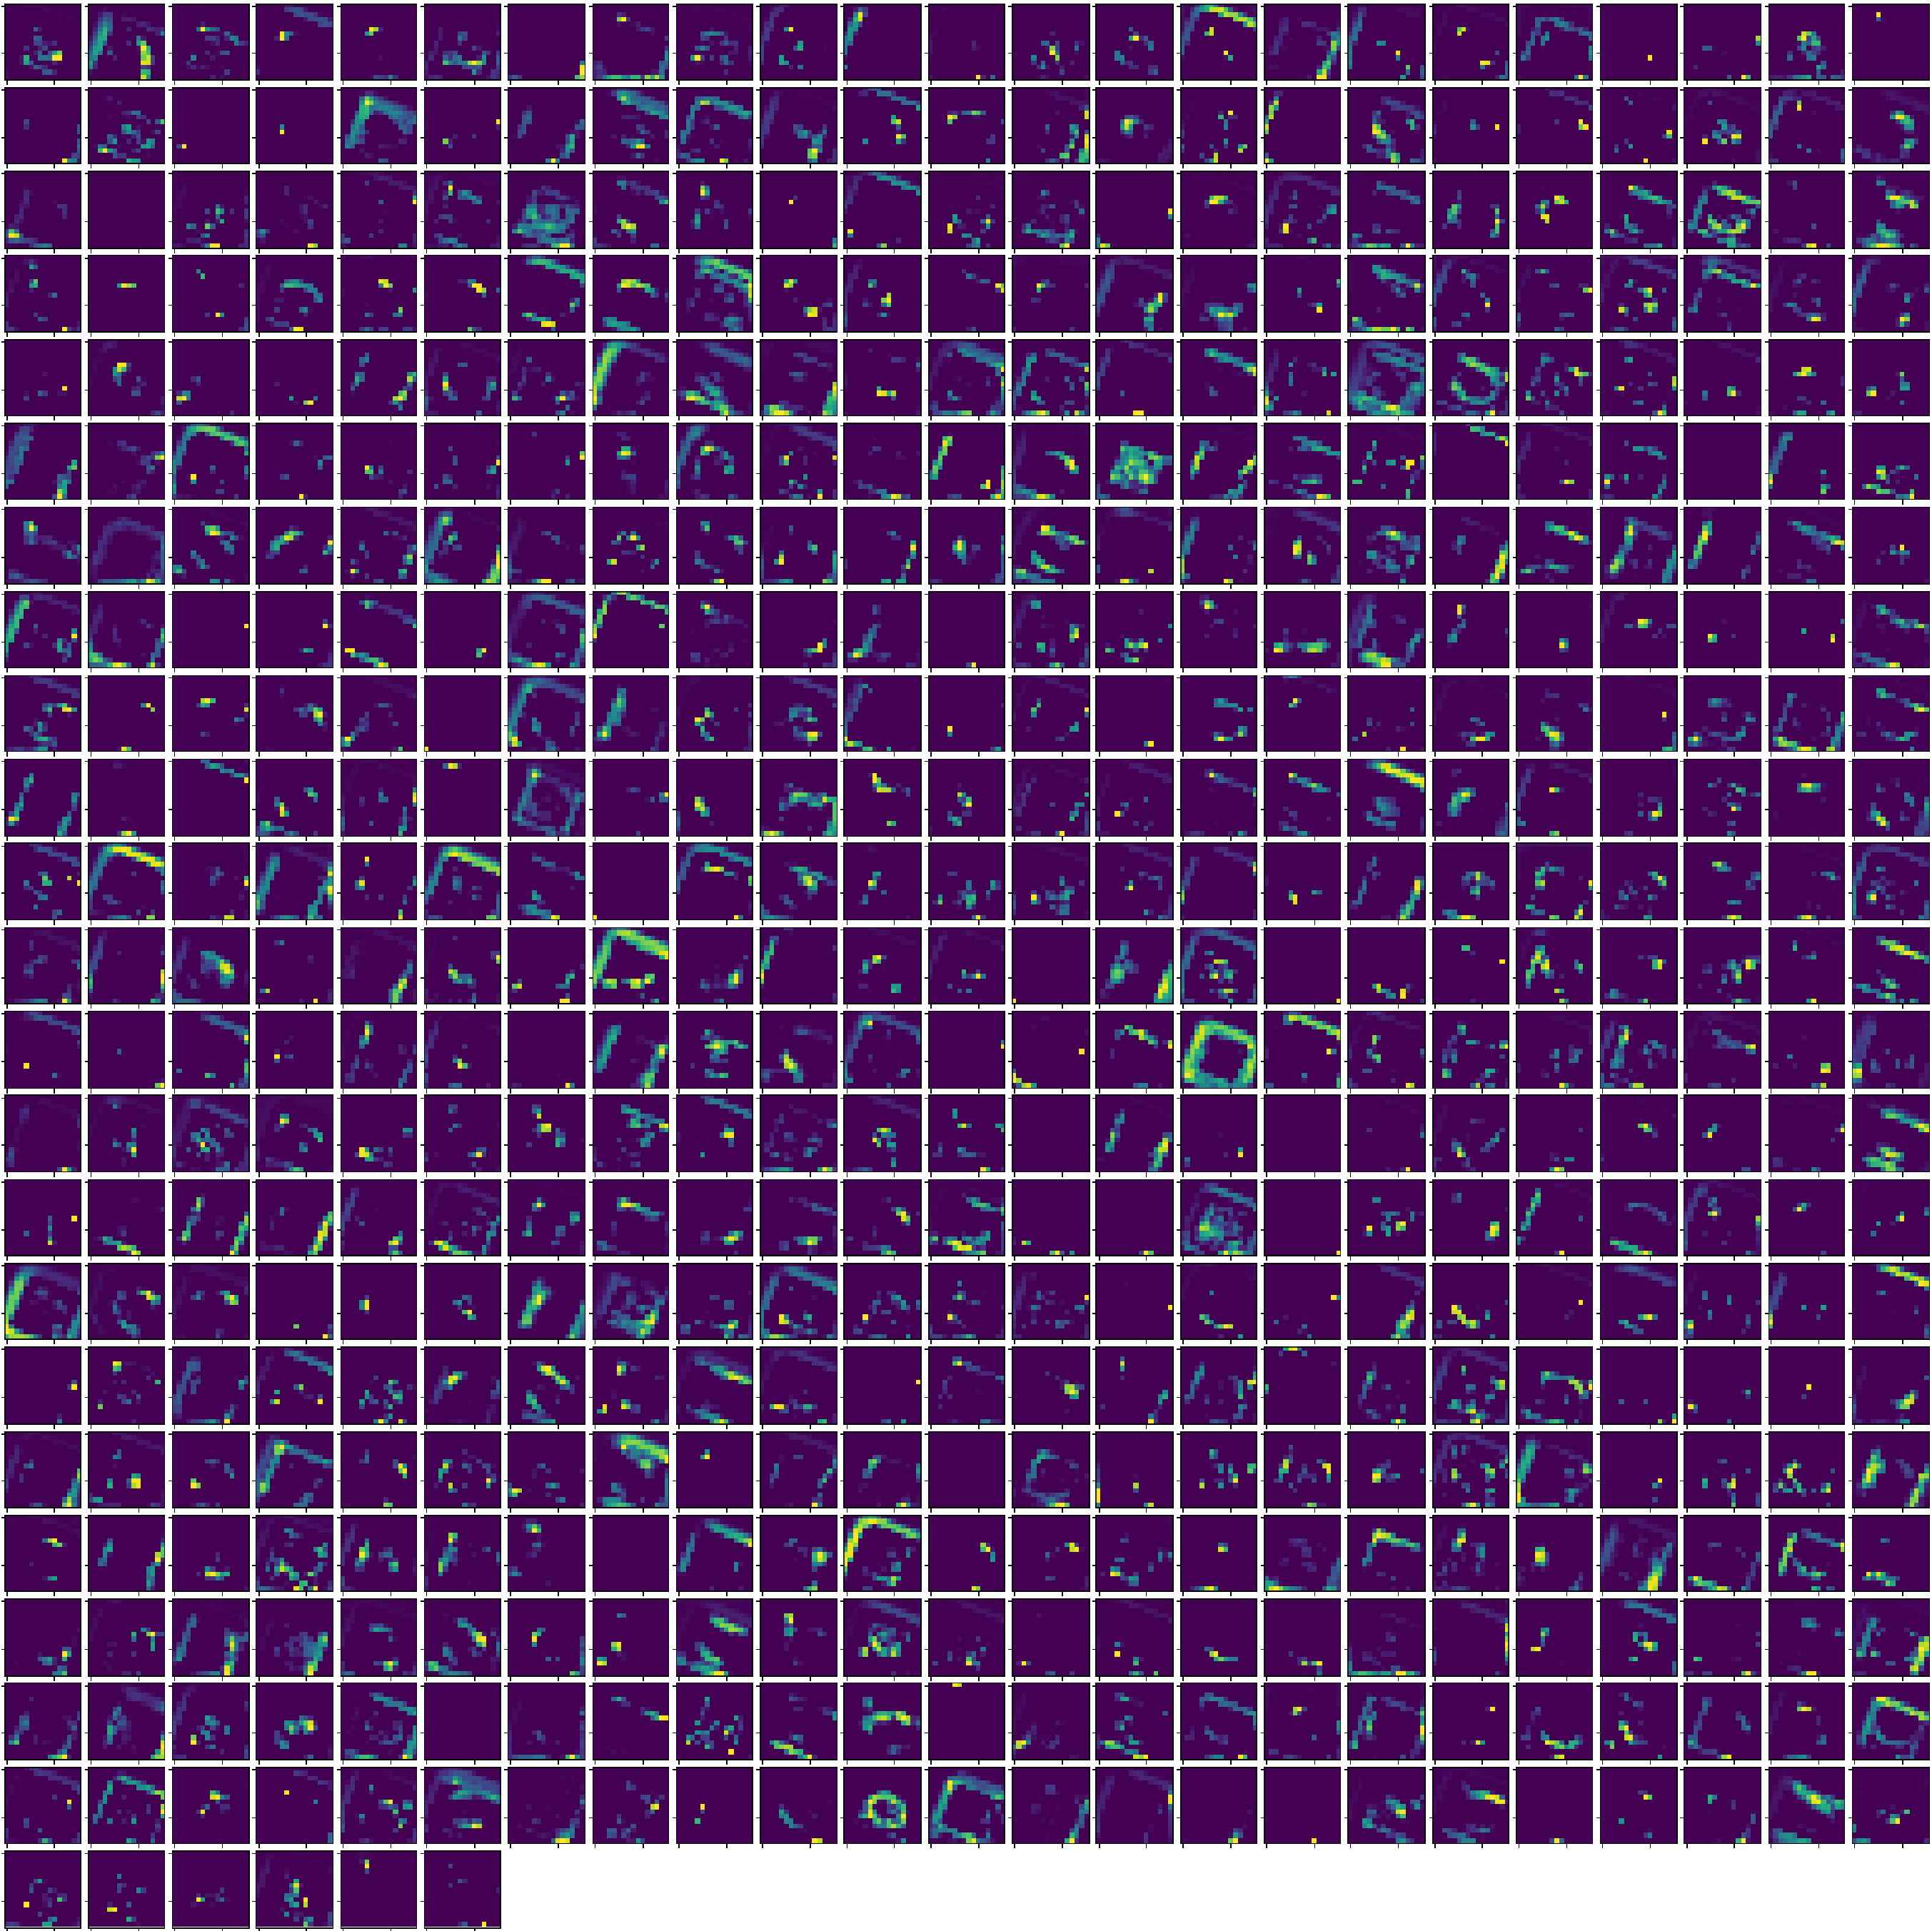
\includegraphics[width=\linewidth]{capitulo_sdac/xcancerblock4_pool-MaxPool_0.pdf}
      \caption{Block4\_pool}\label{fig:ey}
    \end{subfigure}\hspace*{\fill}
    \begin{subfigure}{0.40\textwidth}
      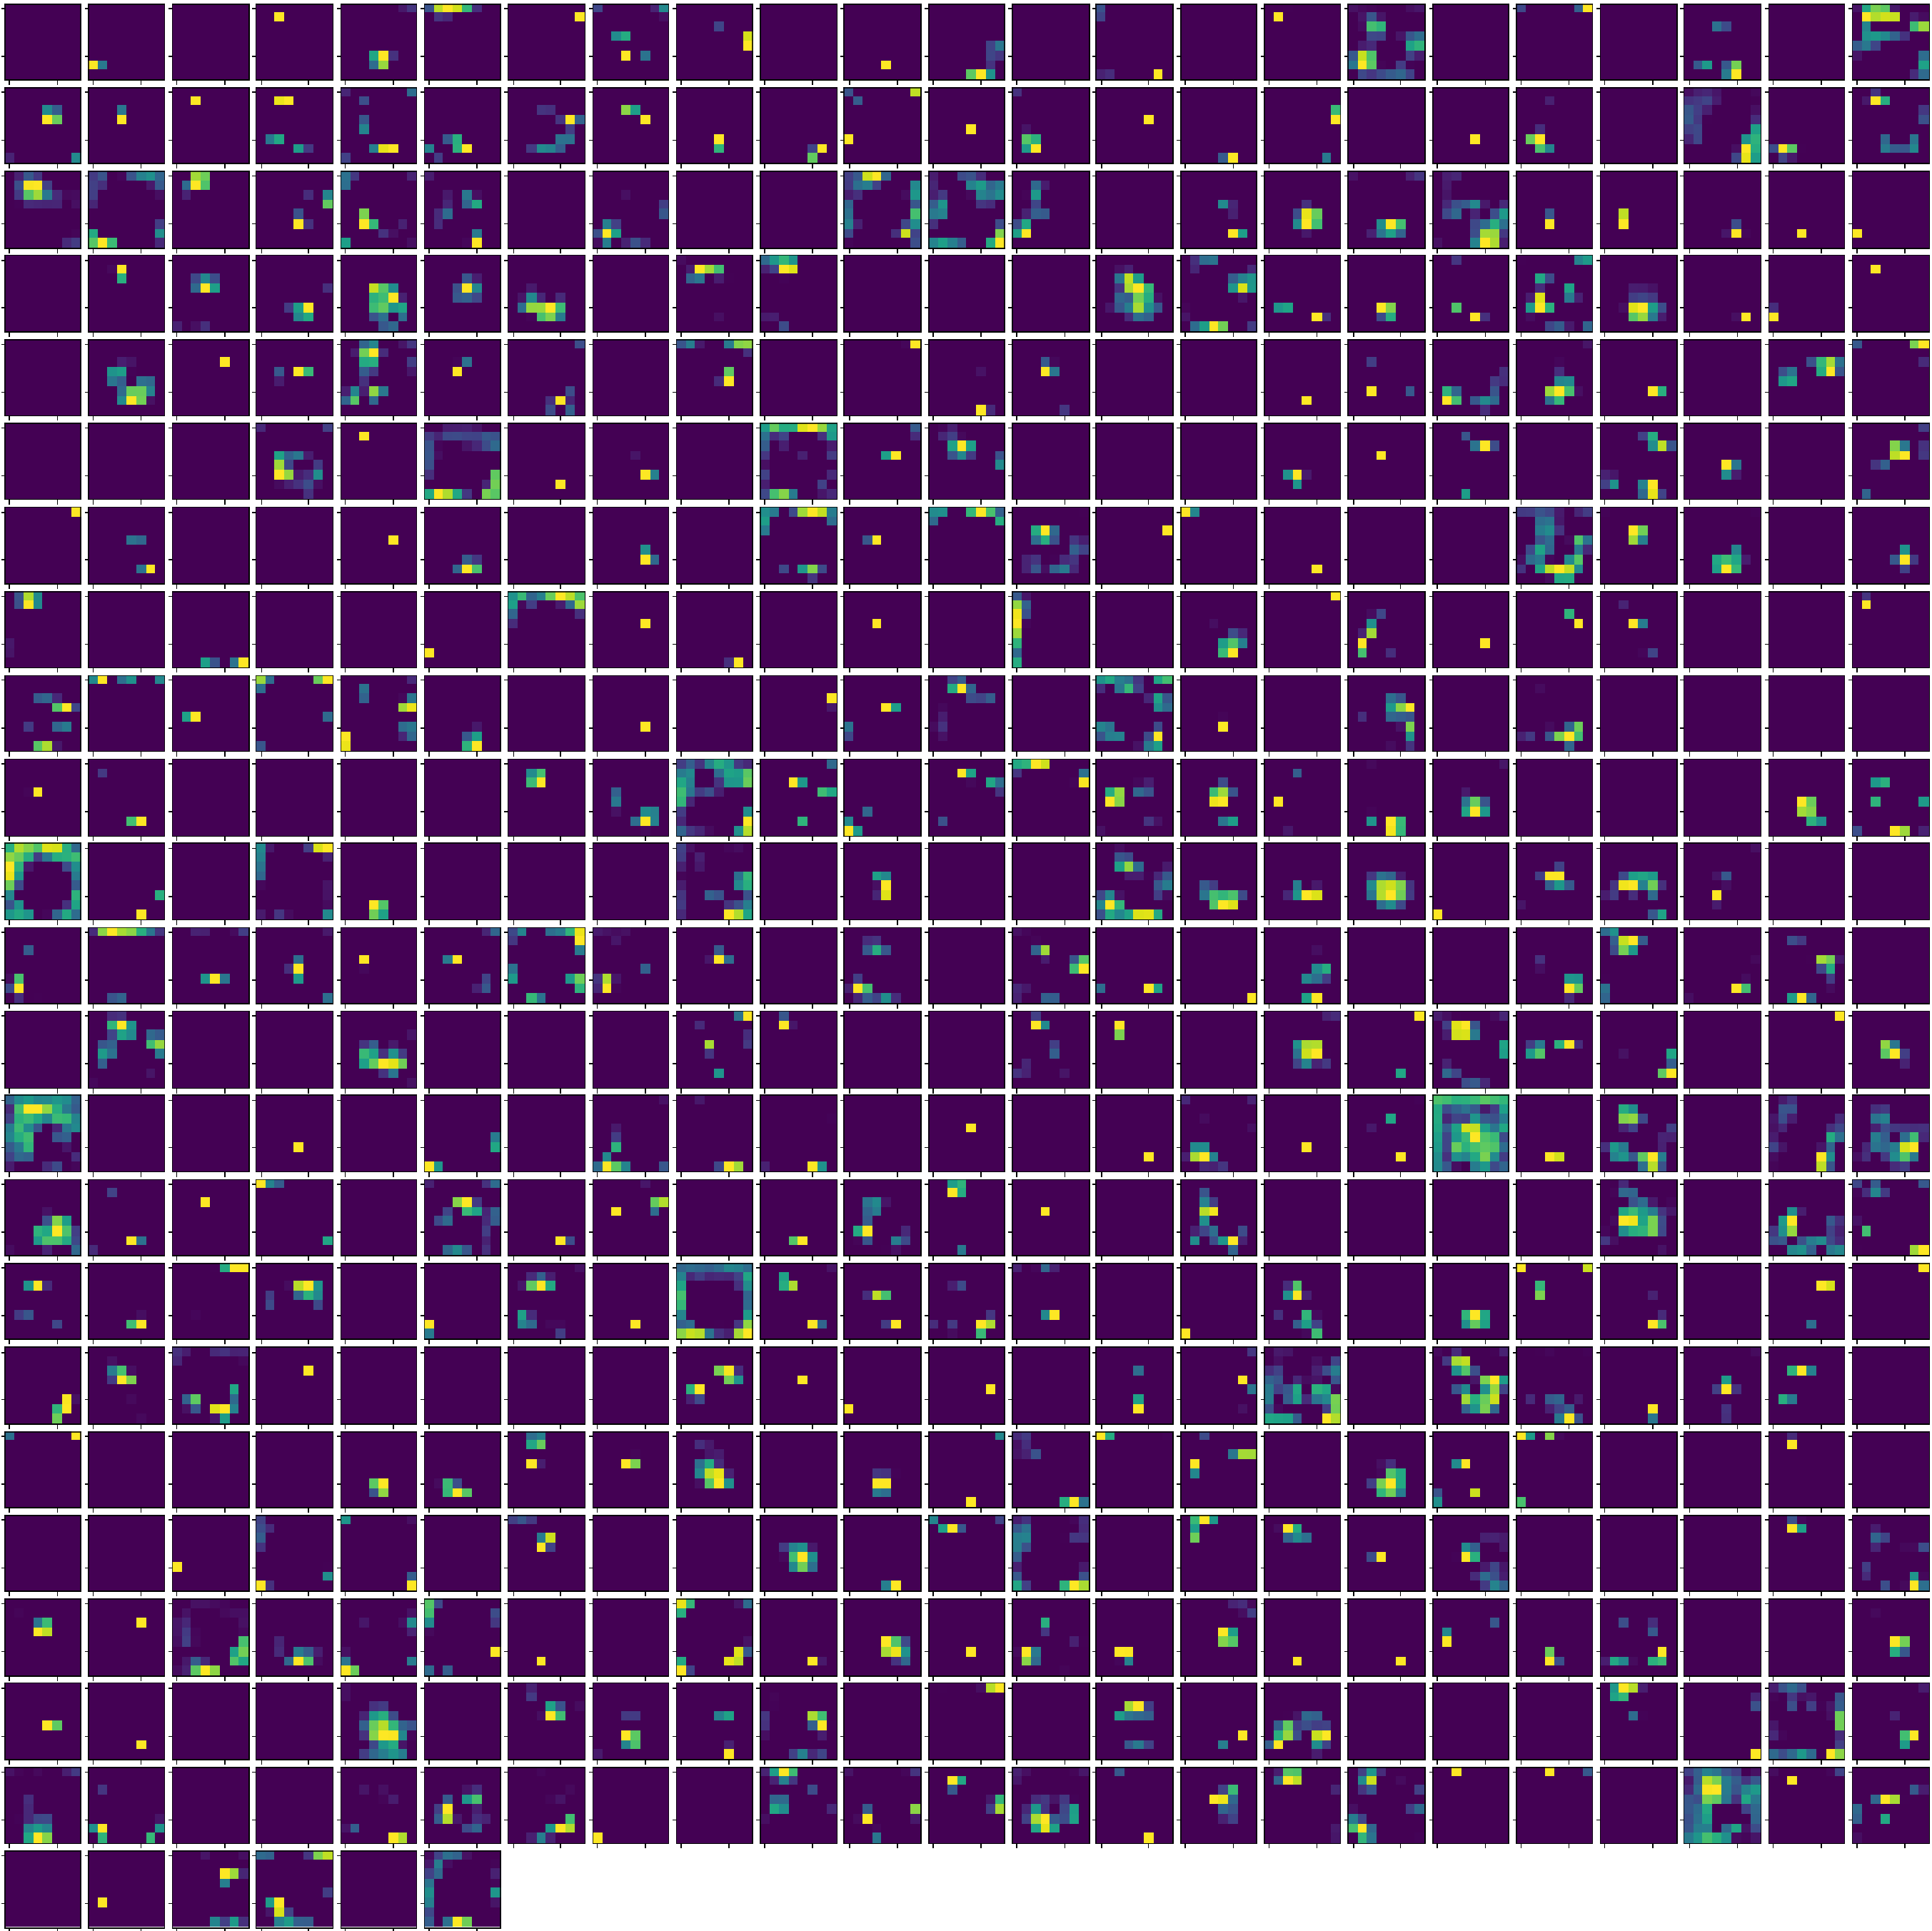
\includegraphics[width=\linewidth]{capitulo_sdac/xcancerblock5_pool-MaxPool_0.pdf}
      \caption{Block5\_pool}\label{fig:fy}
    \end{subfigure}
    \caption{Activaciones de capas \emph{MaxPool} intermedias con entrada de célula cancerígena}\label{fig:inter}
    \end{figure}

Las activaciones en la última capa, si bien son bastante abstractas, ofrecen
atisbos sobre lo que está buscando la red para clasificar cada clase
(\autoref{fig:densa}). En algunas clases, sobre todo las normales, se observa un
claro patrón que se puede interpretar como un núcleo. Mientras que las anormales
tienen a der más caóticas, aunque se pueden distinguir ciertas estructuras
circulares en ellas.

\begin{figure}[H]
    \centering
    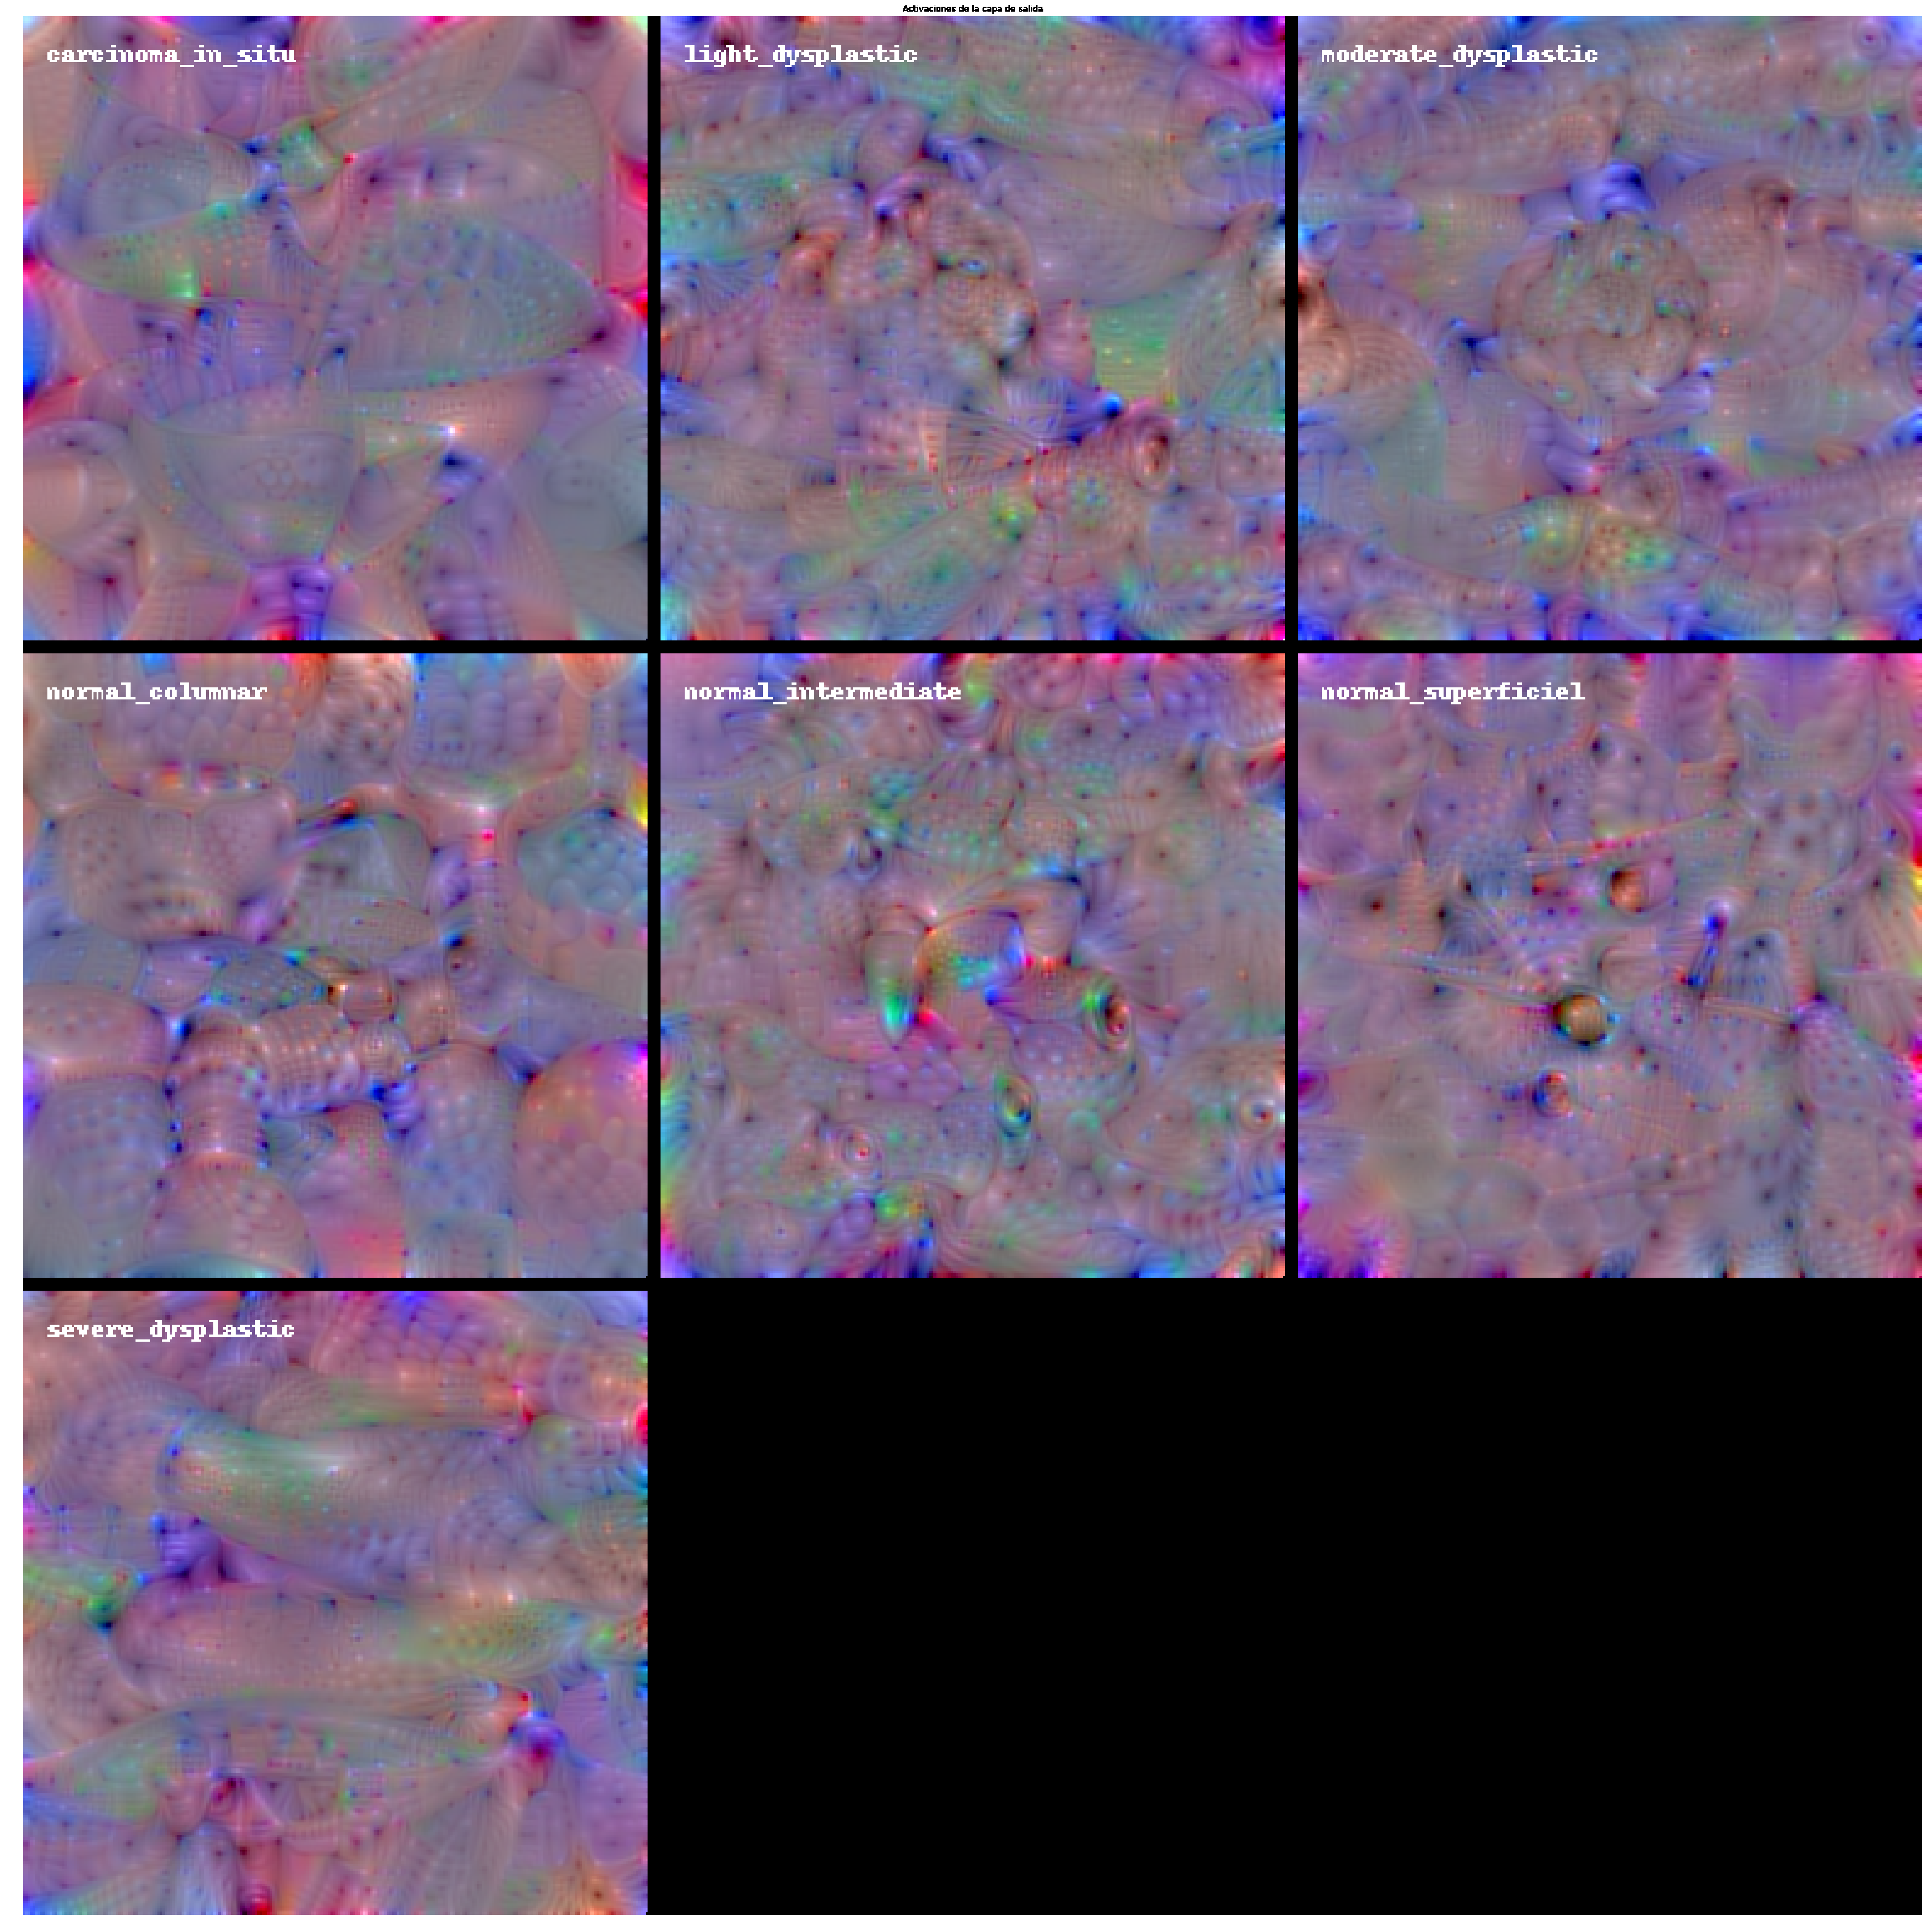
\includegraphics[width=0.8\textwidth]{capitulo_sdac/activacion candidato1.pdf}
    \caption{Visualizaciones de la última capa densa para 7 clases}\label{fig:densa}
\end{figure}

\subsubsection{Análisis de supuestos}

Las técnicas de visualización nos permiten ver y analizar lo que aprende una
ConvNet, modelos que generalmente se han tomado como una caja negra debido a su
complejidad.

Estos algoritmos buscan encontrar, dada cierta entrada y una posterior
optimización por gradiente, que partes de la imagen fueron usadas por la red
neuronal para clasificar. Lo que nos permitirá observar si efectivamente el
núcleo forma parte de la clasificación y si el aumento de datos incide en la
misma.

El método es estocástico e iterativo, cierta variación y discrepancia es de
esperarse. También se cuenta con tres variantes de cada método que por si solas
no ofrecen la claridad buscada, en consecuencia se aplicarán todas en la
comparativa. Estos mapas nos permiten determinar el grado de importancia en la
decisión de cada pixel que compone la imagen.

Se tomaron aleatoriamente siete muestras de las siete clases para las
comparativas.

La~\autoref{fig:saliency} se compone de las imágenes muestra y los mapas
respectivos. ReLU nos permite ver que las decisiones fueron tomadas en base al
contenido de la imagen y los pixeles negros añadidos durante el proceso de
aumentación de datos no influyeron en la decisión. El método normal nos muestra
que los pixeles usados para la decisión fueron aquellos pertenecientes al núcleo
celular. Finalizando con el método guiado que confirma que el núcleo fue el
factor de decisión; aunque el método induce cierto ruido que se manifiesta en
los bordes, los otros no tienen este comportamiento.

  \begin{figure}[H] 
    \begin{subfigure}[b]{0.5\linewidth}
      \centering
      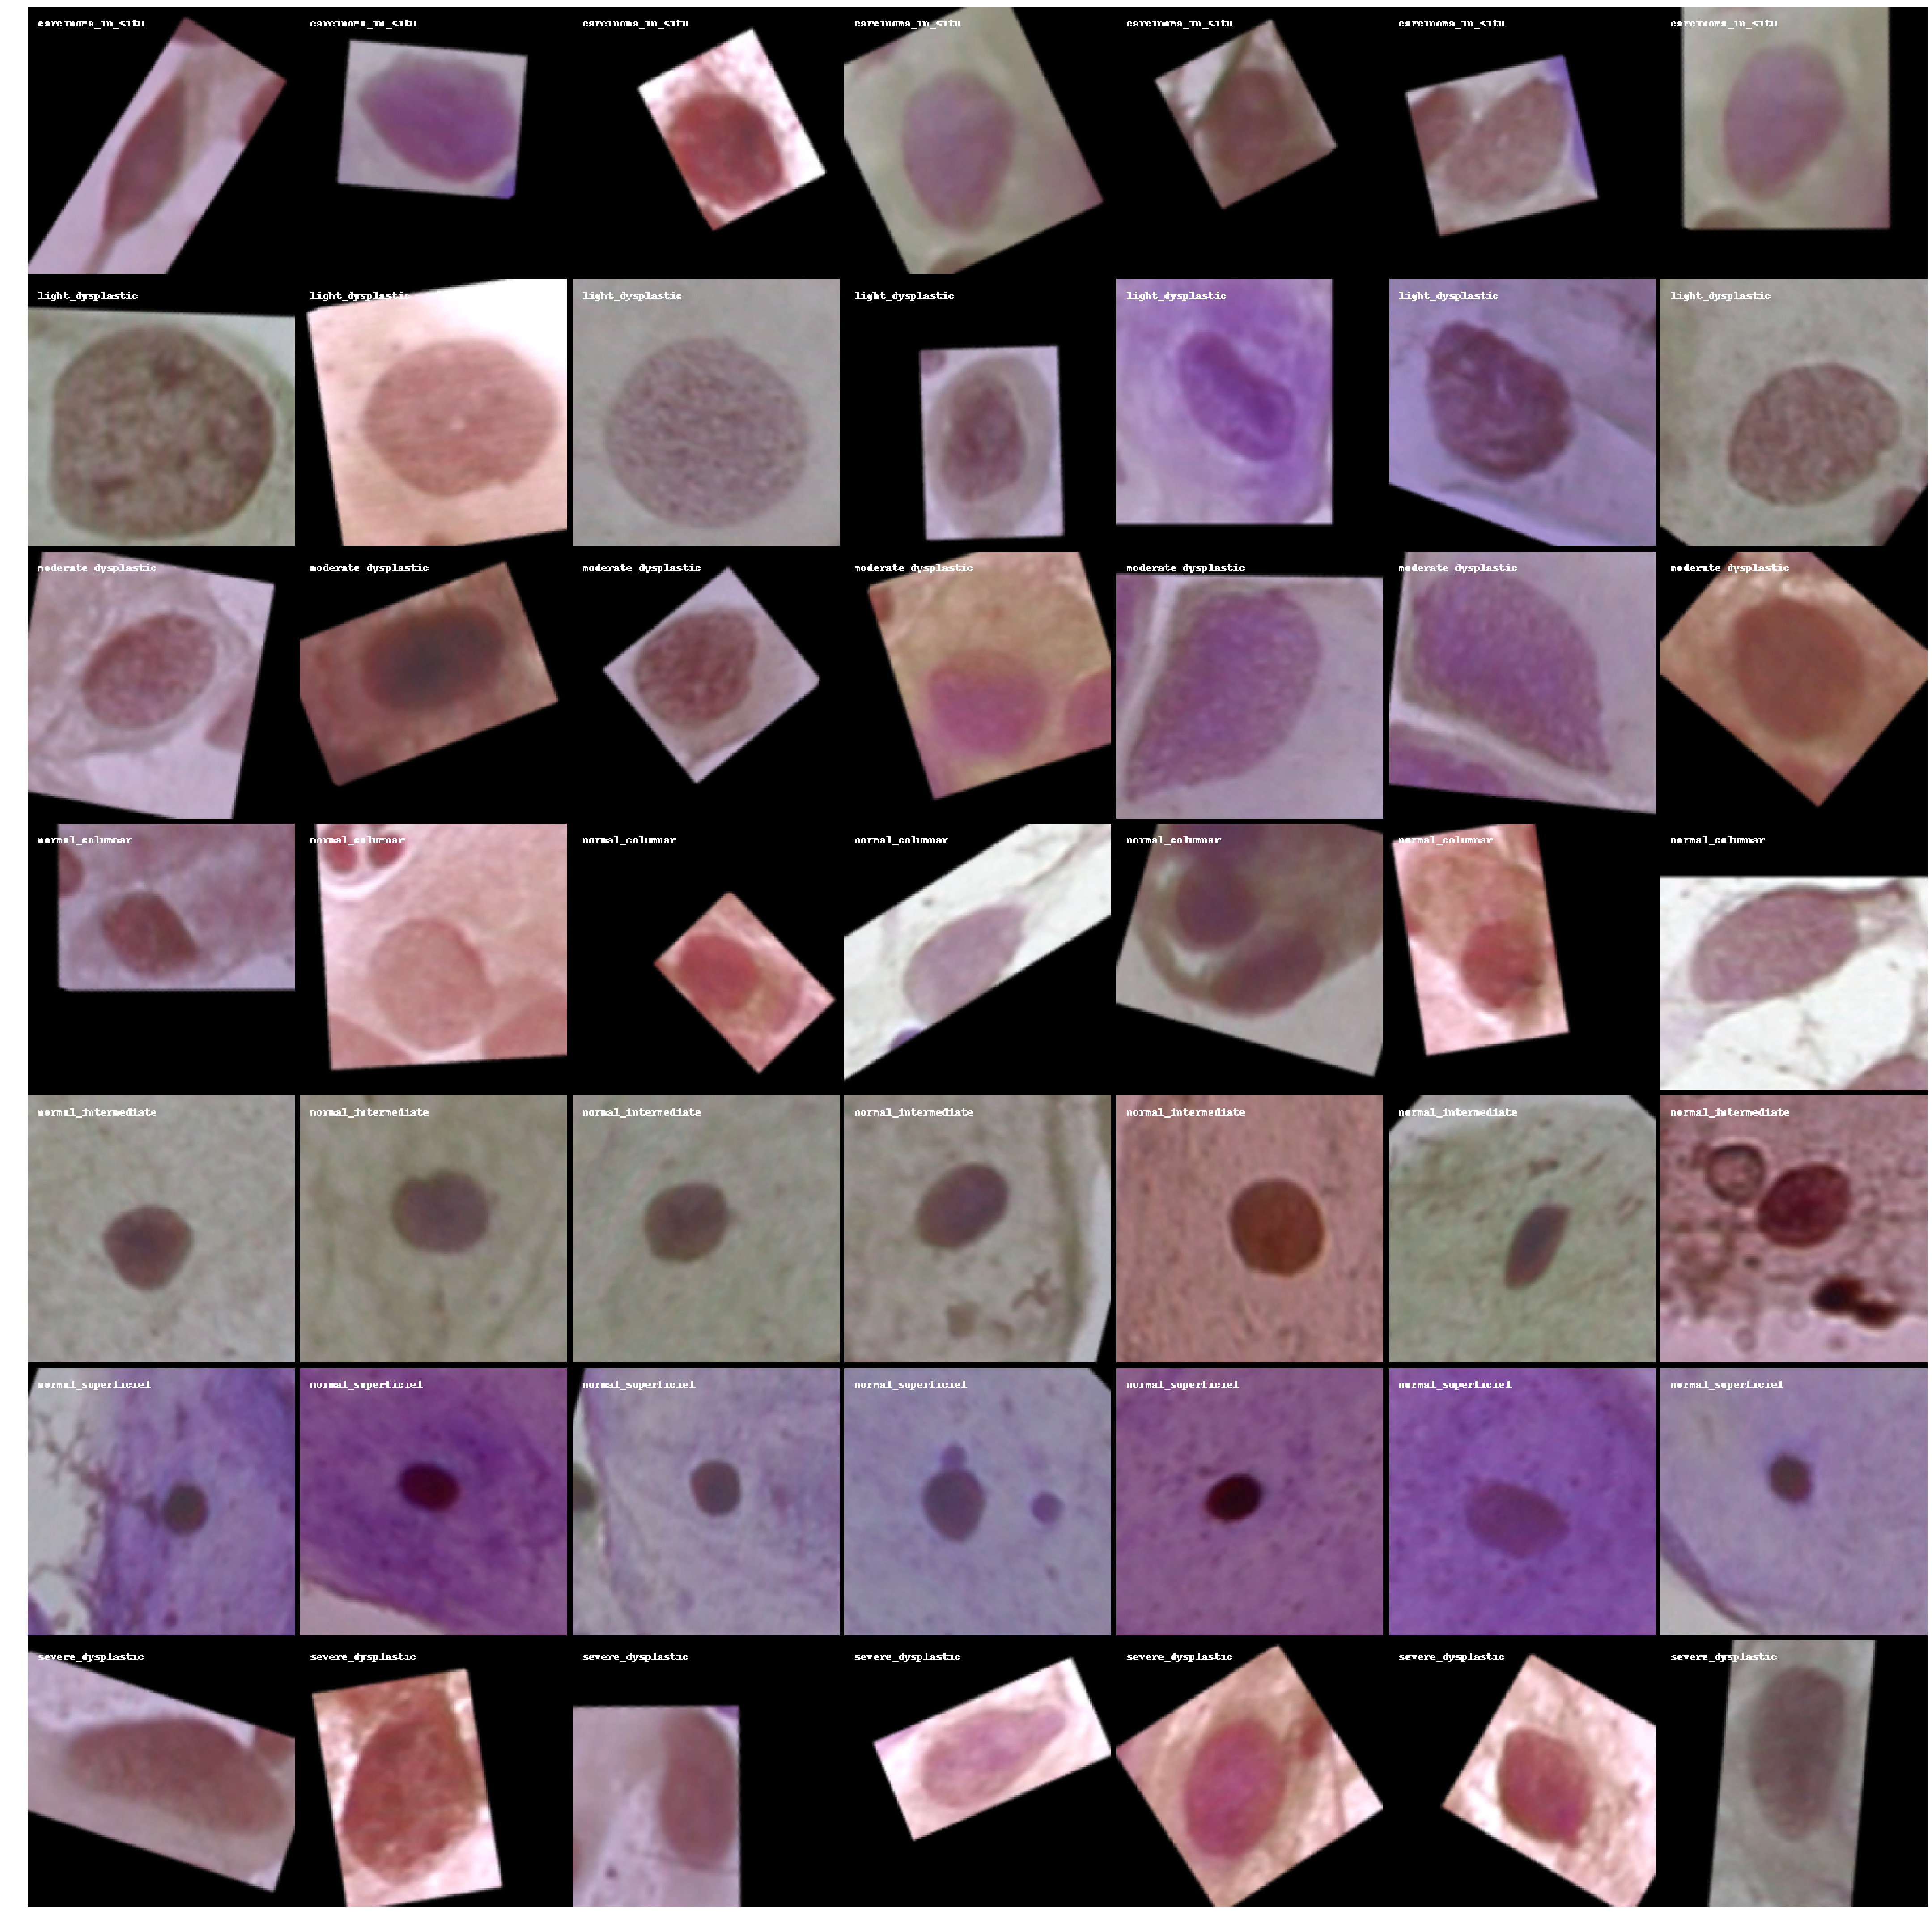
\includegraphics[width=0.75\linewidth]{capitulo_sdac/muestras_saliency.pdf} 
      \caption{Muestras}\label{fig7:a} 
      \vspace{4ex}
    \end{subfigure}%% 
    \begin{subfigure}[b]{0.5\linewidth}
      \centering
      \includegraphics[width=0.75\linewidth]{capitulo_sdac/saliency_relu.pdf} 
      \caption{Prominencia ReLU}\label{fig7:b} 
      \vspace{4ex}
    \end{subfigure} 
    \begin{subfigure}[b]{0.5\linewidth}
      \centering
      \includegraphics[width=0.75\linewidth]{capitulo_sdac/saliency_normal.pdf} 
      \caption{Prominencia normal}\label{fig7:c} 
    \end{subfigure}%%
    \begin{subfigure}[b]{0.5\linewidth}
      \centering
      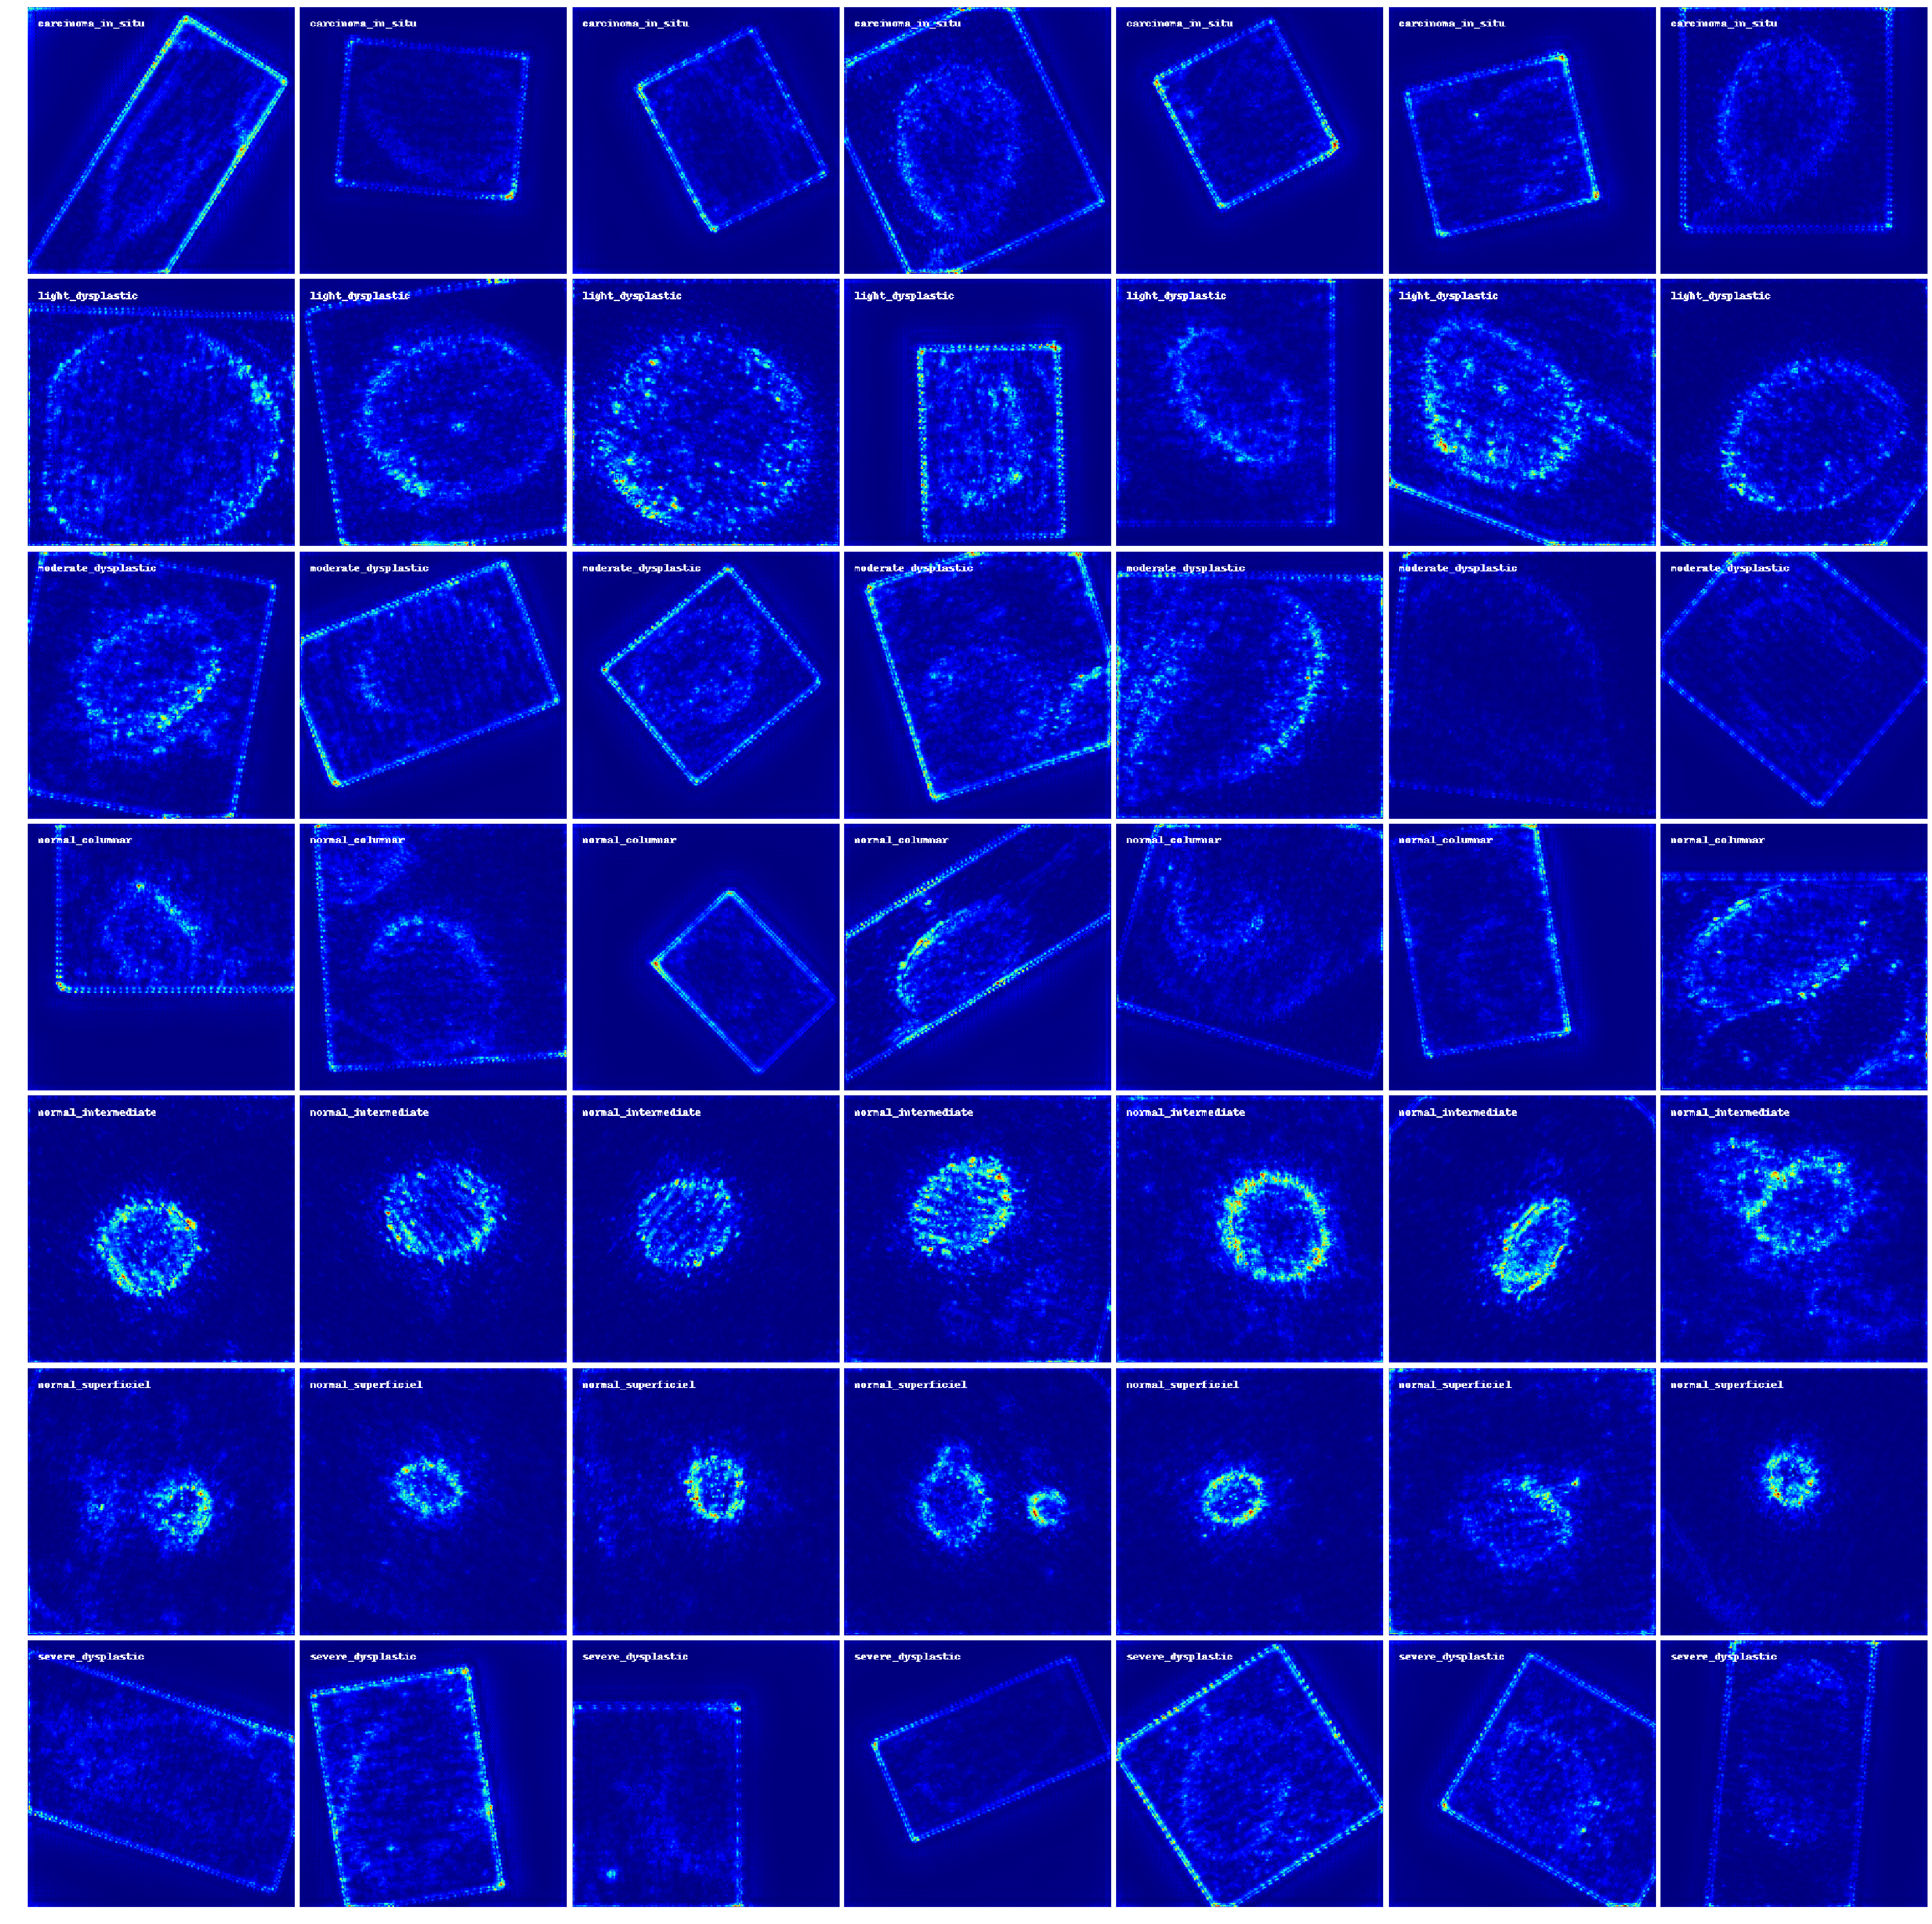
\includegraphics[width=0.75\linewidth]{capitulo_sdac/saliency_guided.pdf} 
      \caption{Prominencia guided}\label{fig7:d} 
    \end{subfigure} 
    \caption{Visualización de mapas de prominencia y comparativa}\label{fig:saliency} 
  \end{figure}

  El método \emph{Gradient-weighted Class Activation Mapping} genera una máscara
  que es superpuesta en la imagen de activación para ver que parte de la imagen
  contribuyó más a la activación. La~\autoref{fig:cam} nos muestra estos
  gradientes de activación para las muestras. Podemos ver que,
  satisfactoriamente, la parte con mayor peso en la activación se concentra en
  el núcleo. Debido a la naturaleza del modelo y su inicialización aleatoria y
  de optimización, estas activaciones no siempre se interceptan el núcleo exacto,
  pero sin duda alguna este fue el que culminó la toma de decisión de la capa.

  \begin{figure}[H] 
      \begin{subfigure}[b]{0.5\linewidth}
        \centering
        \includegraphics[width=0.75\linewidth]{capitulo_sdac/muestras_saliency.pdf} 
        \caption{Muestras}\label{fig7:ab}
        \vspace{4ex}
      \end{subfigure}%% 
      \begin{subfigure}[b]{0.5\linewidth}
        \centering
        \includegraphics[width=0.75\linewidth]{capitulo_sdac/cam_relu.pdf} 
        \caption{Cam ReLU}\label{fig7:ba}
        \vspace{4ex}
      \end{subfigure} 
      \begin{subfigure}[b]{0.5\linewidth}
        \centering
        \includegraphics[width=0.75\linewidth]{capitulo_sdac/cam_normal.pdf} 
        \caption{Cam normal}\label{fig7:cd}
      \end{subfigure}%%
      \begin{subfigure}[b]{0.5\linewidth}
        \centering
        \includegraphics[width=0.75\linewidth]{capitulo_sdac/cam_guided.pdf} 
        \caption{Cam guided}\label{fig7:dc}
      \end{subfigure} 
      \caption{Grad-CAM: Gradient-weighted Class Activation Mapping y muestras de comparativa}\label{fig:cam} 
    \end{figure}

Las pruebas de oclusión, como otras técnicas de visualización, nos permiten ver que pixeles de
una imagen se activan más al momento de evaluar tal imagen para su clasificación. La diferencia
radica en que, en oclusión, se crea un obstáculo de \(m \times n\) y se mueve secuencialmente
a través de la imagen para determinar tanto los pixeles de activación como la robustez del
algoritmo a la oclusión, es decir, que el objeto a buscar se encuentre oculto tras otro. 

La~\autoref{fig:oclusion} son los resultados de la prueba, para la cual se tomaron
aleatoriamente una imagen de cada clase. Podemos observar que efectivamente el 
algoritmo se enfoca en el núcleo y los resultados de consecutivas iteraciones del proceso
de oclusión arrojan que también es robusto antes esta prueba de estrés.
  \begin{figure}[H] % "[t!]" placement specifier just for this example
    \begin{subfigure}{0.40\textwidth}
    \includegraphics[width=\linewidth]{capitulo_sdac/occlusion-carcinoma_in_situ0.pdf}
    \caption{Oclusión para \emph{carcinoma\_in\_situ}}\label{fig:a}
    \end{subfigure}\hspace*{\fill}
    \begin{subfigure}{0.40\textwidth}
    \includegraphics[width=\linewidth]{capitulo_sdac/occlusion-light_dysplastic13.pdf}
    \caption{Oclusión para \emph{light\_dysplastic}}\label{fig:b}
    \end{subfigure}
    
    \medskip
    \begin{subfigure}{0.40\textwidth}
    \includegraphics[width=\linewidth]{capitulo_sdac/occlusion-moderate_dysplastic25.pdf}
    \caption{Oclusión para \emph{moderate\_dysplastic}}\label{fig:cc}
    \end{subfigure}\hspace*{\fill}
    \begin{subfigure}{0.40\textwidth}
    \includegraphics[width=\linewidth]{capitulo_sdac/occlusion-normal_columnar34.pdf}
    \caption{Oclusión para \emph{normal\_columnar}}\label{fig:dd}
    \end{subfigure}
    
    \medskip
    \begin{subfigure}{0.40\textwidth}
    \includegraphics[width=\linewidth]{capitulo_sdac/occlusion-normal_intermediate44.pdf}
    \caption{Oclusión para \emph{normal\_intermediate}}\label{fig:c}
    \end{subfigure}\hspace*{\fill}
    \begin{subfigure}{0.40\textwidth}
    \includegraphics[width=\linewidth]{capitulo_sdac/occlusion-normal_superficiel59.pdf}
    \caption{Oclusión para \emph{normal\_superficiel}}\label{fig:d}
    \end{subfigure}

    % \hspace*{\fill}
    \centering
    \begin{subfigure}{0.40\textwidth}
      
    \includegraphics[width=\linewidth]{capitulo_sdac/occlusion-severe_dysplastic64.pdf}
    \caption{Oclusión para \emph{severe\_dysplastic}}\label{fig:e}
    \end{subfigure}
    
    \caption{Prueba de oclusión para todas las clases}\label{fig:oclusion}
    \end{figure}
    
Para comprobar el último supuesto, necesitaremos aplicar técnicas de reducción
de dimensionalidad. De todas las técnicas de reducción de dimensionalidad en la
actualidad, \hyperlink{abbr}{t-SNE} es el
que ha dado mejores resultados a la hora de visualizar datos multidimensionales
extraídos de las capas de una red neuronal. Este algoritmo está implementado en
\textbf{Python}

Los hiper-parámetros utilizados para correr el algoritmo se muestra a
continuación en la \autoref{fig:hiper_tsne}. Se hicieron pruebas manuales para
encontrar el mejor nivel de \emph{perplexity}. La implementación del algoritmo
en \textbf{Python} es paralelizada, por lo que se pudieron usar todos los
núcleos disponibles del sistema. 

\begin{figure}[H]
    \centering
\begin{minted}{python}
                            PERPLEXITY = 2000
                            N_JOBS = 16
\end{minted}
\caption{Hiperparámetros para \emph{t-SNE}}\label{fig:hiper_tsne}
\end{figure}

Se tomaron los datos de validación usados para la mejor iteración de la
validación cruzada y se alimentaron al algoritmo \hyperlink{abbr}{t-SNE}
(\autoref{fig:tsne}). Podemos ver que todas las clases están correctamente
separadas en racimos. La diferencia de forma entre los racimos nos da evidencia
de la complejidad de la imagen con relación a la clase que representa.

\begin{itemize}
  \item{\emph{normal\_superficiel:}} Se encuentra bien diferenciada, con algunos valores que se varían
  más que el resto.
  \item{\emph{normal\_intermediate:}} Igual que la anterior, un racimo bien diferenciado con pocos valores
  variantes.
  \item{\emph{normal\_columnar:}} Podemos ver que existen dos subclases dentro de esta clase y que
  se diferencian por ciertas características morfológicas, observamos también como algunas células
  \emph{severe\_dysplastic} y \emph{carcinoma\_in\_situ} se catalogan erróneamente en esta clase.
  \item{\emph{light\_dysplastic:}} Estas células están agrupadas en forma de media luna lo cual
  muestra que son más complejas de agrupar.
  \item{\emph{moderate\_dysplastic:}} Encontramos en este racimo algunas células mal clasificadas.
  \item{\emph{severe\_dysplastic:}} Varias células de \emph{carcinoma\_in\_situ} son mal
  clasificadas dentro de esta clase, lo cual nos muestra una progresión directa entre una
  clase a otra.
  \item{\emph{carcinoma\_in\_situ:}} Se encuentran bien diferenciadas y no se confunden con
  ninguna normal.
\end{itemize}

\begin{figure}[H]
    \centering
    \includegraphics[width=0.90\textwidth]{capitulo_sdac/tsne-7clases3-84954-2000.pdf}
    \caption{Reducción de dimensionalidad con t-sne}\label{fig:tsne}
\end{figure}

Podemos ver que el algoritmo puede clasificar correctamente y los resultados de
la reducción de la dimensionalidad son consistentes con las métricas de
evaluación para un modelo de clasificación. Habiendo tintes células anormales en
la clase \emph{normal\_columnar} mientras que las otras dos clases normales
están correctamente separadas del resto.

\subsection{Modelo}

El problema de clasificación de imágenes de índole citológica, en particular a
las células encontradas dentro de una laminilla de examen \hyperlink{abbr}{PAP}, pertenece
a la categoría de problemas que pueden ser resueltos mediante \hyperlink{abbr}{DL},
utilizando \hyperlink{abbr}{ConvNet}s.

Como se mostró en el Estado del Arte, a la fecha existen varios intentos de
clasificación de células para examen \hyperlink{abbr}{PAP}.
La~\autoref{tabla:comparativa2} muestra el rendimiento de clasificación de
distintos métodos, con sus respectivas métricas, para el problema de dos clases.
También se incluyen en la comparativa los resultados de las tesis y los
artículos de la \hyperlink{abbr}{BD} de Herlev, que funge como benchmark.

Solamente el penúltimo, \emph{DeepPap}, utiliza \hyperlink{abbr}{DL}, los otros
son métodos tradicionales que conjugan Extracción de Características y otros
algoritmos de Machine Learning. La comparativa demuestra la superioridad del
método de solución que se propone en la tesis, teniendo mejor rendimiento y
menor variación. El trabajo de esta tesis se validó usando validación cruzada de
10 iteraciones, lo cual hace una mejor estimación del error de generalización y
provee mejor balance entre el sesgo y la varianza, en comparación a usar 5
iteraciones; por ello el benchmark usa 10.

\begin{table}[H]
  \centering
  \resizebox{\textwidth}{!}{%
  \begin{tabular}{@{}lllllll@{}}
  \toprule
  Métodos & k-fold CV & TPR/Sens & TNR/Spec & ACC & F1 & AUC \\ \midrule
  Benchmark & 10 & \(98.8 \pm 1.3\) & \(79.3 \pm 6.3\) & \(93.6 \pm 1.9\) & 88.0 &\- \\
  PSO-lnn & 5 & 98.4 & 92.2 & 96.7 & 95.2 & - \\
  GEN-lnn & 5 & 98.5 & 92.1 & 96.8 & 95.2 &\ - \\
  ANN & - & 99.9 & 96.5 & 99.3 & 98.2 & - \\
  K-PCA + SVM & 5 & - & - & - & 96.9 & - \\
  Ensemble & 5 & 99 & 89.7 & 96.5 & - & - \\
  Ens & 5 & - & - & - & - & 0.884 \\
  dis(S+M) & 5 & - & - & - & - & 0.964 \\
  DeepPap & 5 & \(98.2 \pm 1.2\) & \(98.3 \pm 0.9\) & \(98.3 \pm 0.7\) & \(98.3 \pm 0.3\) & 0.998 \\
  Tesis2 & 10 & \(\mathbf{0.99857}\) & \(\mathbf{0.99979}\) & \(\mathbf{99.86}\) & \(\mathbf{0.99918}\) & \textbf{0.99918} \\ \bottomrule
  \end{tabular}%
  }
  \caption{Comparativa para el problema binario}\label{tabla:comparativa2}
  \end{table}

\emph{DeepPap} también realiza pruebas para el problema de siete
clases, y nos ofrece una exactitud total de 98.5\%, mientras que el método de
solución para siete clases propuesto en esta tesis, alcanza 99.58\%. El error
total de \emph{DeepPap} queda en 1.6\%, mientras que la tesis tiene uno de
0.42\%, lo cual nos dice la red entrenada en los experimentos realizados
en este trabajo es más de tres veces mejor que el competidor más cercano. 
